\documentclass{article}
\usepackage[utf8]{inputenc}
\usepackage{amsmath}
\usepackage{graphicx}
\usepackage{array}
\usepackage{booktabs}
\usepackage{float}
\usepackage{caption}
\usepackage{subcaption}
\usepackage{xcolor, colortbl}
\usepackage{lscape}
\usepackage{array, multirow, multicol}
\usepackage[margin=2.5cm]{geometry}
\usepackage{fancyhdr, parskip}
\usepackage[hidelinks]{hyperref}
\usepackage{fancyhdr, parskip}
\usepackage{tikz}
\usetikzlibrary{arrows.meta, fit, backgrounds}
\renewcommand*\contentsname{Index}

\fancyhead[R]{
    
\includegraphics[width = 2.5cm]{UA (color) C.jpg}
}

\title{Cloud Computing Services}
\author{Raúl Boix Aldeguer 77953850L\\Alejandro Benito Marcos}
\date{September 2026}


\begin{document}

\maketitle
\thispagestyle{fancy}
\newpage
\tableofcontents
\newpage

\section{Introduction}
    \subsection{Objectives}

    This practice develops a Smart City application for a Smart Lighting System (SLS): a controller that switches the lights of an urban area on or off depending on whether people or vehicles are present in the control zone. Using cameras as presence sensors avoids keeping the lights on all night when nobody is around, which reduces energy consumption. Code is in \href{https://github.com/Parka1/AIIA-Practice1}{\textcolor{blue}{Github}}.

    Frames from a public webcam are used as the input of the system, and a person detection model decides whether the zone is occupied. The main goal is to learn how to offload this AI processing to the cloud and to evaluate the advantages and drawbacks of doing so. In particular, the specific objectives are:

    \begin{itemize}
        \item Build a frame capture process for a public webcam and a common format to store detection results.
        \item Count people in each frame with YOLOv8, first on a local machine and then on an Azure virtual machine (IaaS).
        \item Implement a serverless version on Azure, using a blob-triggered Azure Function and the Azure AI Vision service.
        \item Measure and compare the three architectures in terms of detection efficiency, response time, resource usage, bandwidth and monetary cost.
        \item Study how each architecture scales when the number of cameras increases.
    \end{itemize}


    \subsection{System Overview}

    Figure~\ref{fig:overview} summarizes the architecture of the system. A capture process running on a local machine obtains a frame from a public webcam every 5 seconds. The frame is then processed in one of three ways, each corresponding to one part of the practice:

    \begin{itemize}
        \item \textbf{Local processing (Part 1):} the YOLOv8 model runs on the local machine itself, and the people count of each frame is stored in a CSV file and plotted over time.
        \item \textbf{Cloud virtual machine (Part 2, IaaS):} the frame is sent over HTTP to an Azure virtual machine, which runs YOLOv8. Then it stores the results and creates a web page with the statistics available via a public IP address.
        \item \textbf{Serverless (Part 3):} the frame is uploaded to a \texttt{raw} Blob Storage container. Each upload triggers an Azure Function that sends the image to the Azure AI Vision service, draws the bounding boxes of the detected people and publishes the results on a static website hosted in the \texttt{\$web} container.
    \end{itemize}

    All three architectures share the same capture module and write their results in the same CSV format. Each frame is identified by the same \texttt{frame\_id}, so the results of the different architectures can be compared frame by frame.

    In a real deployment, the lighting controller would use the number of detected people to switch the lights on or off, depending on a fixed threshold.

    \begin{figure}[h]
      \centering
      \resizebox{\textwidth}{!}{%
      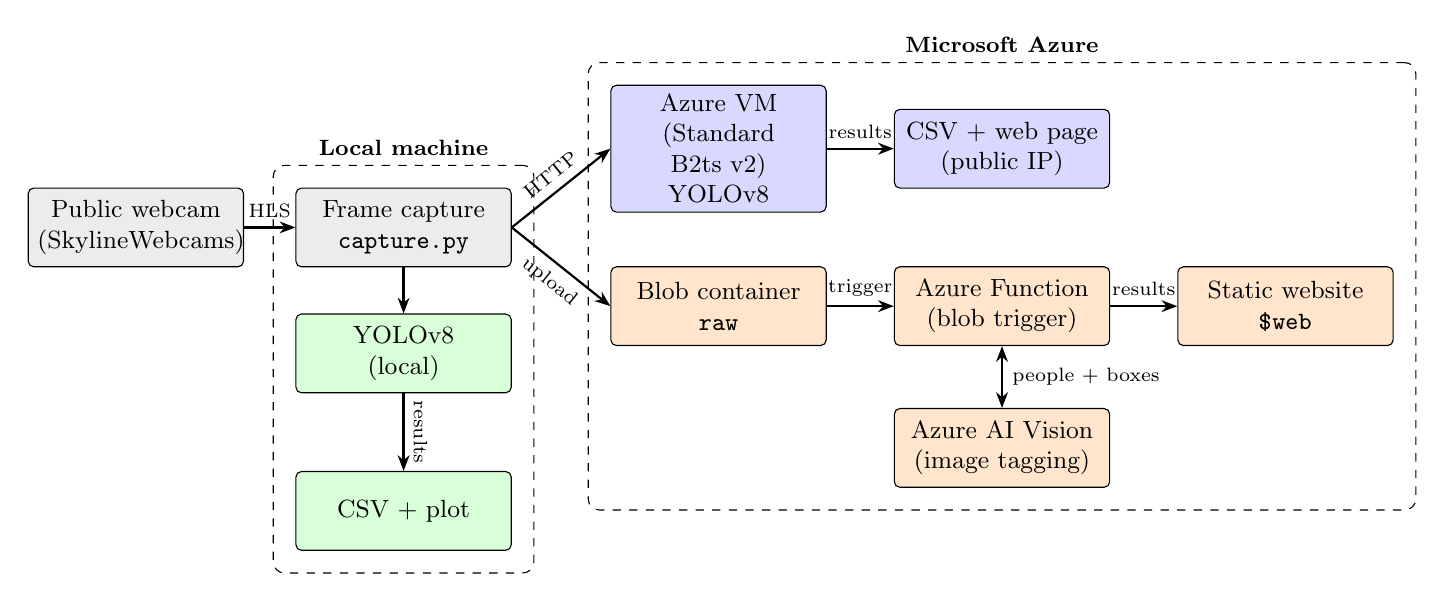
\begin{tikzpicture}[
          box/.style={draw, rounded corners=2pt, align=center, text width=2.5cm,
                      minimum height=1cm, font=\small},
          shared/.style={box, fill=gray!15},
          p1/.style={box, fill=green!15},
          p2/.style={box, fill=blue!15},
          p3/.style={box, fill=orange!20},
          group/.style={draw, dashed, rounded corners=4pt, inner sep=8pt},
          arr/.style={-{Stealth[length=2mm]}, thick},
          lbl/.style={font=\scriptsize, midway, above, sloped},
        ]
        % Shared components
        \node[shared] (cam) at (0,0.6)   {Public webcam\\(SkylineWebcams)};
        \node[shared] (cap) at (3.4,0.6) {Frame capture\\\texttt{capture.py}};

        % Part 1: local
        \node[p1] (yolo) at (3.4,-1.0) {YOLOv8\\(local)};
        \node[p1] (plot) at (3.4,-3.0) {CSV + plot};

        % Part 2: VM
        \node[p2] (vm)    at (7.4,1.6)  {Azure VM (Standard B2ts v2)\\YOLOv8};
        \node[p2] (vmweb) at (11.0,1.6) {CSV + web page\\(public IP)};

        % Part 3: serverless
        \node[p3] (raw)    at (7.4,-0.4)  {Blob container\\\texttt{raw}};
        \node[p3] (func)   at (11.0,-0.4) {Azure Function\\(blob trigger)};
        \node[p3] (vision) at (11.0,-2.2) {Azure AI Vision\\(image tagging)};
        \node[p3] (web)    at (14.6,-0.4) {Static website\\\texttt{\$web}};

        % Arrows
        \draw[arr] (cam) -- node[lbl]{HLS} (cap);
        \draw[arr] (cap) -- (yolo);
        \draw[arr] (yolo) -- node[lbl]{results} (plot);
        \draw[arr] (cap.east) -- node[lbl]{HTTP} (vm.west);
        \draw[arr] (cap.east) -- node[lbl, below]{upload} (raw.west);
        \draw[arr] (vm) -- node[lbl]{results} (vmweb);
        \draw[arr] (raw) -- node[lbl]{trigger} (func);
        \draw[{Stealth[length=2mm]}-{Stealth[length=2mm]}, thick]
            (func) -- node[midway, right, font=\scriptsize]{people + boxes} (vision);
        \draw[arr] (func) -- node[lbl]{results} (web);

        % Groups
        \begin{scope}[on background layer]
          \node[group, fit=(cap)(yolo)(plot),
                label={[font=\footnotesize\bfseries]above:Local machine}] {};
          \node[group, fit=(vm)(vmweb)(raw)(func)(vision)(web),
                label={[font=\footnotesize\bfseries]above:Microsoft Azure}] {};
        \end{scope}
      \end{tikzpicture}%
      }
      \caption{System overview. Grey: components shared by all architectures. Green: local processing (Part 1). Blue: cloud virtual machine (Part 2). Orange: serverless architecture (Part 3).}
      \label{fig:overview}
    \end{figure}


\section{Common Components}

All three architectures share the same input (a public webcam), the same frame capture code and the same output format. These components are in the \texttt{common/} folder of the repository and are described in this section.

    \subsection{Webcam Selection (Task 1.1)}

    The initial camera was the SkylineWebcams camera on the \emph{Paseo Marítimo} of Santa Pola (Alicante)\footnote{\url{https://www.skylinewebcams.com/es/webcam/espana/comunidad-valenciana/santa-pola/paseo-maritimo.html}}, shown in Figure~\ref{fig:webcam}. It was chosen because it shows a street with a pedestrian crossing, a promenade and restaurants, so both people and vehicles are present during all day. It streams at 1920$\times$1080.

    The scene also has drawbacks that affect detection. The street has parking spaces on both sides, so most of the vehicles in each frame are parked. Only moving vehicles should be detected (as we do not want parked vehicles to turn on the lights), so these parked vehicles have to be filtered out (see Section~\ref{sec:vehicles}). In addition, people at the terraces and in the background are only a few pixels tall and are harder to detect. Santa Pola was retained as the initial camera for Part 1 and the first VM run; the later low detections motivated a test of a less panoramic, more centred plaza view in Grazalema. That decision and the two-camera comparison are described in Part 2.

    \begin{figure}[h]
        \centering
        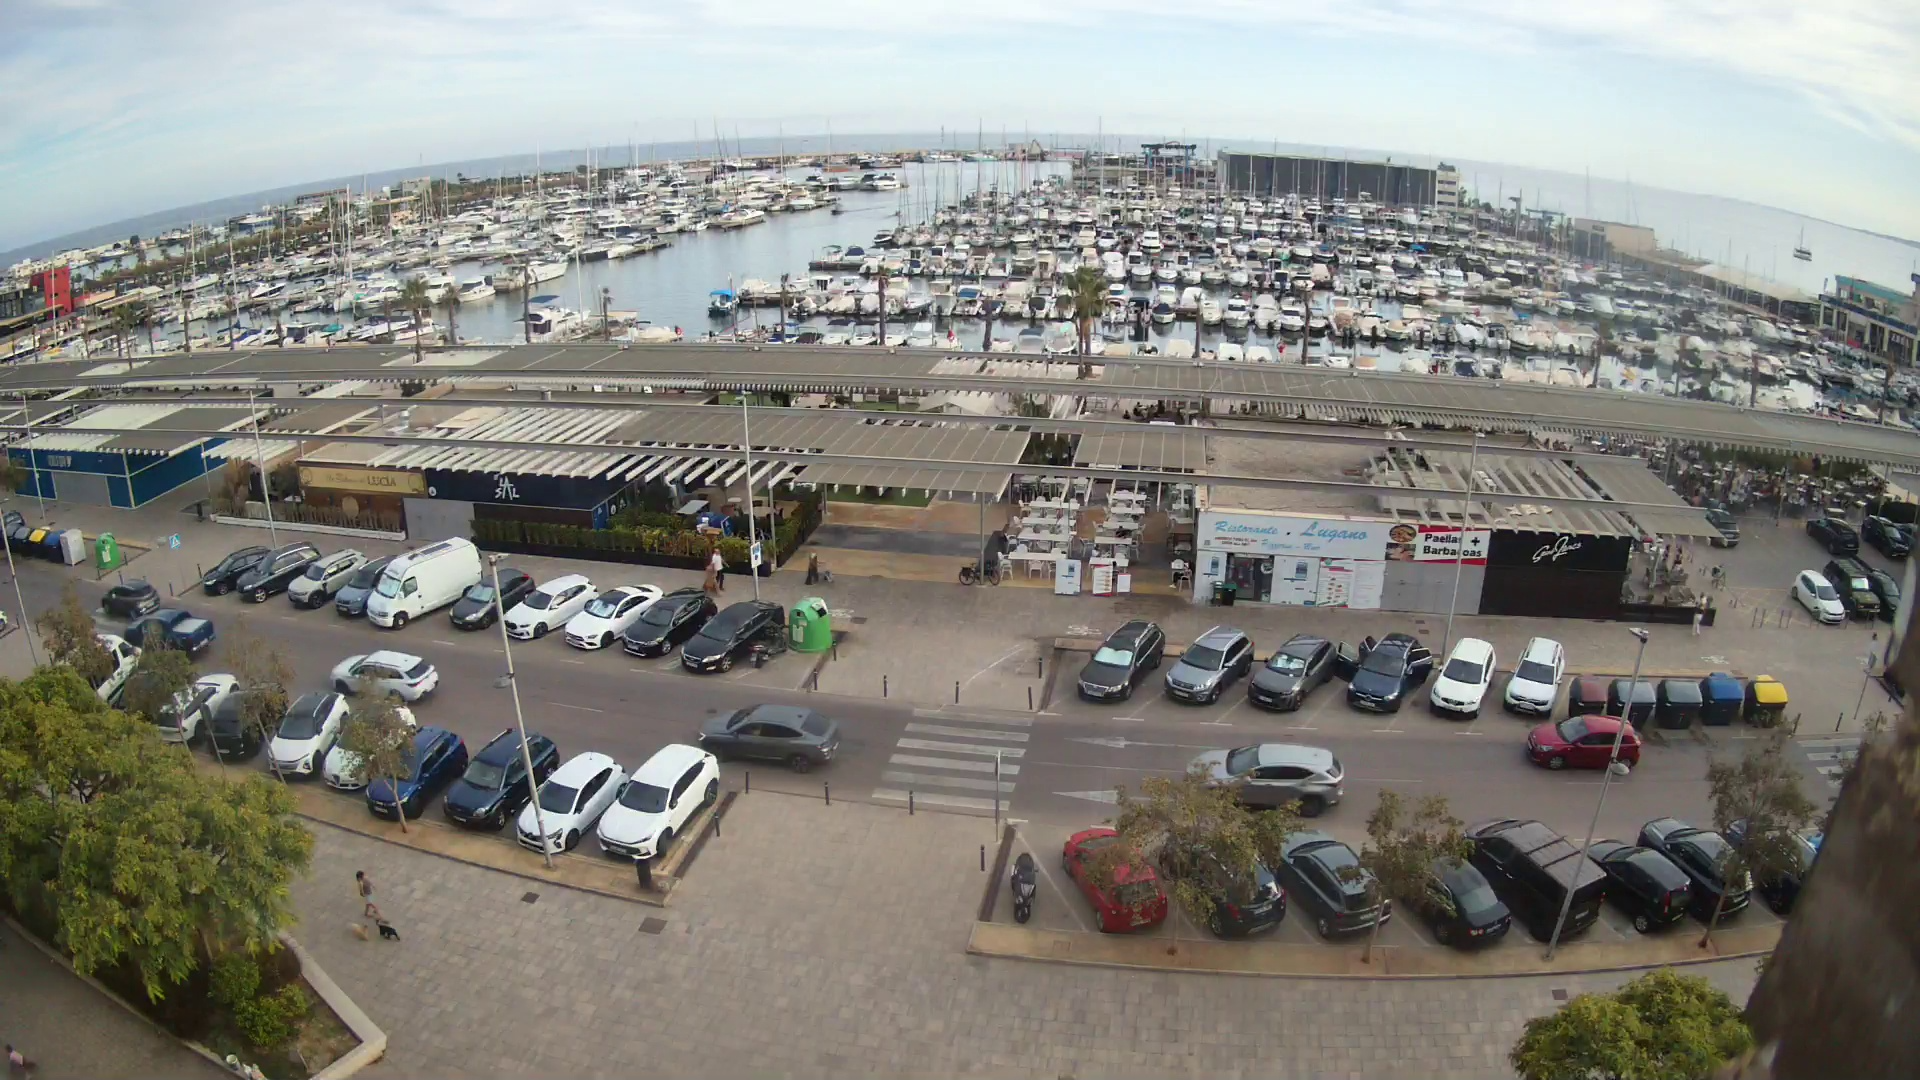
\includegraphics[width=0.8\textwidth]{images/Section_2/santa_pola_frame.jpg}
        \caption{Frame captured from the Santa Pola webcam (1920$\times$1080).}
        \label{fig:webcam}
    \end{figure}

    \subsection{Frame Capture Module (Task 1.2)}

    We capture the images from SkylineWebcams. This web uses HLS (HTTP Live Streaming), a protocol designed to deliver video over plain HTTP: the video is split into short segments of about 3 seconds, listed in a playlist file (\texttt{.m3u8}) that the player downloads periodically. Furthermore, webcams are protected with a temporary token embedded in the camera web page.

    For this reason, a new capture module (\texttt{capture.py}) was written. Its main function, \texttt{get\_frame(cam\_url)}, returns the current frame of a camera as an OpenCV image and is reused by all architectures. For SkylineWebcams cameras, it extracts the stream token from the camera web page, which is downloaded again only when the cached token is older than 60 seconds. It then opens the HLS stream with OpenCV (FFmpeg backend), reads a single frame and closes the stream. In this way, an expired token only makes a single capture fail and is replaced in the next one, and no resources are spent receiving and decoding frames that are not going to be processed.

    \paragraph{Problems encountered.}
    \begin{itemize}
        \item \textbf{Token expiration.} Tokens stop working after 2--4 minutes. The module caches the token for 60 seconds and requests a new one whenever the stream cannot be read.
        \item \textbf{Logo frames.} When the token is invalid, the stream can still be opened and it returns the SkylineWebcams logo instead of the camera image. These frames are detected by their proportion of white pixels: about 87\% in the logo, against about 5\% in real frames, so we put a threshold of 60\%. When it is surpassed, it automatically discards the capture and tries again with a new token.
    \end{itemize}


    \subsection{Common Results Format}
    \label{sec:results-format}

    To compare the architectures, all of them write their results in the same CSV format, defined in \texttt{results.py} (Table~\ref{tab:csv-format}). Each row corresponds to one processed frame.

    \begin{table}[htbp]
        \centering
        \small
        \begin{tabular}{lp{9cm}}
            \toprule
            \textbf{Column} & \textbf{Meaning} \\
            \midrule
            \texttt{timestamp}        & Frame capture time \\
            \texttt{architecture}     & \texttt{local}, \texttt{vm} or \texttt{serverless} \\
            \texttt{cam\_id}          & Camera identifier (e.g. \texttt{santa\_pola}) \\
            \texttt{frame\_id}        & \texttt{<cam\_id>\_<capture time>}, e.g. \texttt{santa\_pola\_20260924T201005123} \\
            \texttt{n\_people}        & Number of people detected \\
            \texttt{n\_vehicles}      & Number of vehicles detected that are not parked (empty if not computed) \\
            \texttt{response\_time\_ms} & End-to-end time from frame capture to result stored \\
            \texttt{inference\_ms}    & Time spent in the model or AI Vision call only \\
            \texttt{frame\_bytes}     & Size of the encoded image sent or processed \\
            \bottomrule
        \end{tabular}
        \caption{Common CSV format of the detection results.}
        \label{tab:csv-format}
    \end{table}


\section{Part 1: Local Processing}
    \subsection{Person Detection with YOLOv8 (Task 1.3)}

    The local processing pipeline is implemented in \texttt{local\_vm/process\_local.py}. It uses the Ultralytics YOLOv8 Nano weights (\texttt{yolov8n.pt}) by default and asks YOLO to return only class 0 (person), with a default confidence threshold of 0.25. The model is loaded once and reused for all frames. The capture module successfully returned a 1920$\times$1080 frame from the Santa Pola webcam.

    The process calls the shared \texttt{get\_frame()} function for the Santa Pola webcam and repeats at five-second intervals. A failed capture is reported and skipped; it does not stop subsequent attempts. The interval, number of frames, camera, weights, confidence and inference image size can be configured through command-line options. The first run downloads the model weights if they are not already present.

    \paragraph{Design decisions and problems encountered.}
    The initial inference size of 640 pixels detected no people in a captured image where pedestrians were visible at a distance. On that same image, raising the inference size to 960 pixels detected one person at confidence 0.31; 1280 pixels also detected one person but took longer (approximately 90 ms versus 54 ms in the warmed-up test). The default was therefore changed to 960 pixels to improve detection of small, distant people without the extra cost of 1280. This is a sample-based tuning decision, not a measured accuracy guarantee; the scene and detections still need to be compared against ground truth.

    The host Python environment did not have the required packages and is managed by Homebrew, so a system-wide pip installation was rejected by PEP 668. Dependencies were installed in an isolated virtual environment instead. The first prediction also took longer because YOLO was warming up; subsequent inference times were substantially lower.

    \subsection{CSV Logging and Time Evolution}

    Each successful inference is appended to \texttt{results/local.csv} using the shared schema in \texttt{common/results.py}. It records the local architecture, camera and frame identifiers, timezone-aware capture timestamp, number of people, inference time and response time. In this implementation, response time measures from the captured frame being returned through inference completion; CSV append time is not included. The vehicle count is left empty because it is outside the scope of Part 1. The graph generator in \texttt{local\_vm/plot\_local.py} reads this CSV and saves the people-per-frame time series to \texttt{results/local\_people\_over\_time.png}; both paths can be overridden.

    On the test machine, the system Python environment was externally managed, so the dependencies were installed in an isolated environment: \texttt{python3 -m venv .venv}, followed by \texttt{.venv/bin/python -m pip install -r local\_vm/requirements.txt}. Run \texttt{.venv/bin/python -m local\_vm.process\_local} and generate the graph with \texttt{.venv/bin/python -m local\_vm.plot\_local}. The process can be stopped with Ctrl+C; completed rows remain in the CSV and can be plotted afterward.

    \subsection{Local Results and Performance}

    An end-to-end run processed three webcam frames at five-second intervals on 29 September 2026. The detected person counts were 0, 0 and 2. The corresponding response times were 476.3 ms, 47.8 ms and 47.1 ms; inference times were 476.3 ms, 47.8 ms and 47.1 ms. The first prediction includes YOLO warm-up and is not representative of steady-state performance. The next two inferences took approximately 47 ms each. These three frames demonstrate that capture, inference, CSV logging and graph generation work together, but they are too small a sample to characterize accuracy or performance. The raw rows are retained in \texttt{data/part1\_local\_results.csv}.

    Figure~\ref{fig:part1-detection} shows a separate example webcam frame with a person detected by YOLOv8 at 960 pixels and confidence 0.31; it is not one of the three frames used for the plot. Figure~\ref{fig:part1-plot} plots the three counts from the CSV. There are three data points at 16:26:39.504, 16:26:44.251 and 16:26:49.269, so the first-to-last elapsed time is about 9.8 seconds.

    \begin{figure}[H]
        \centering
        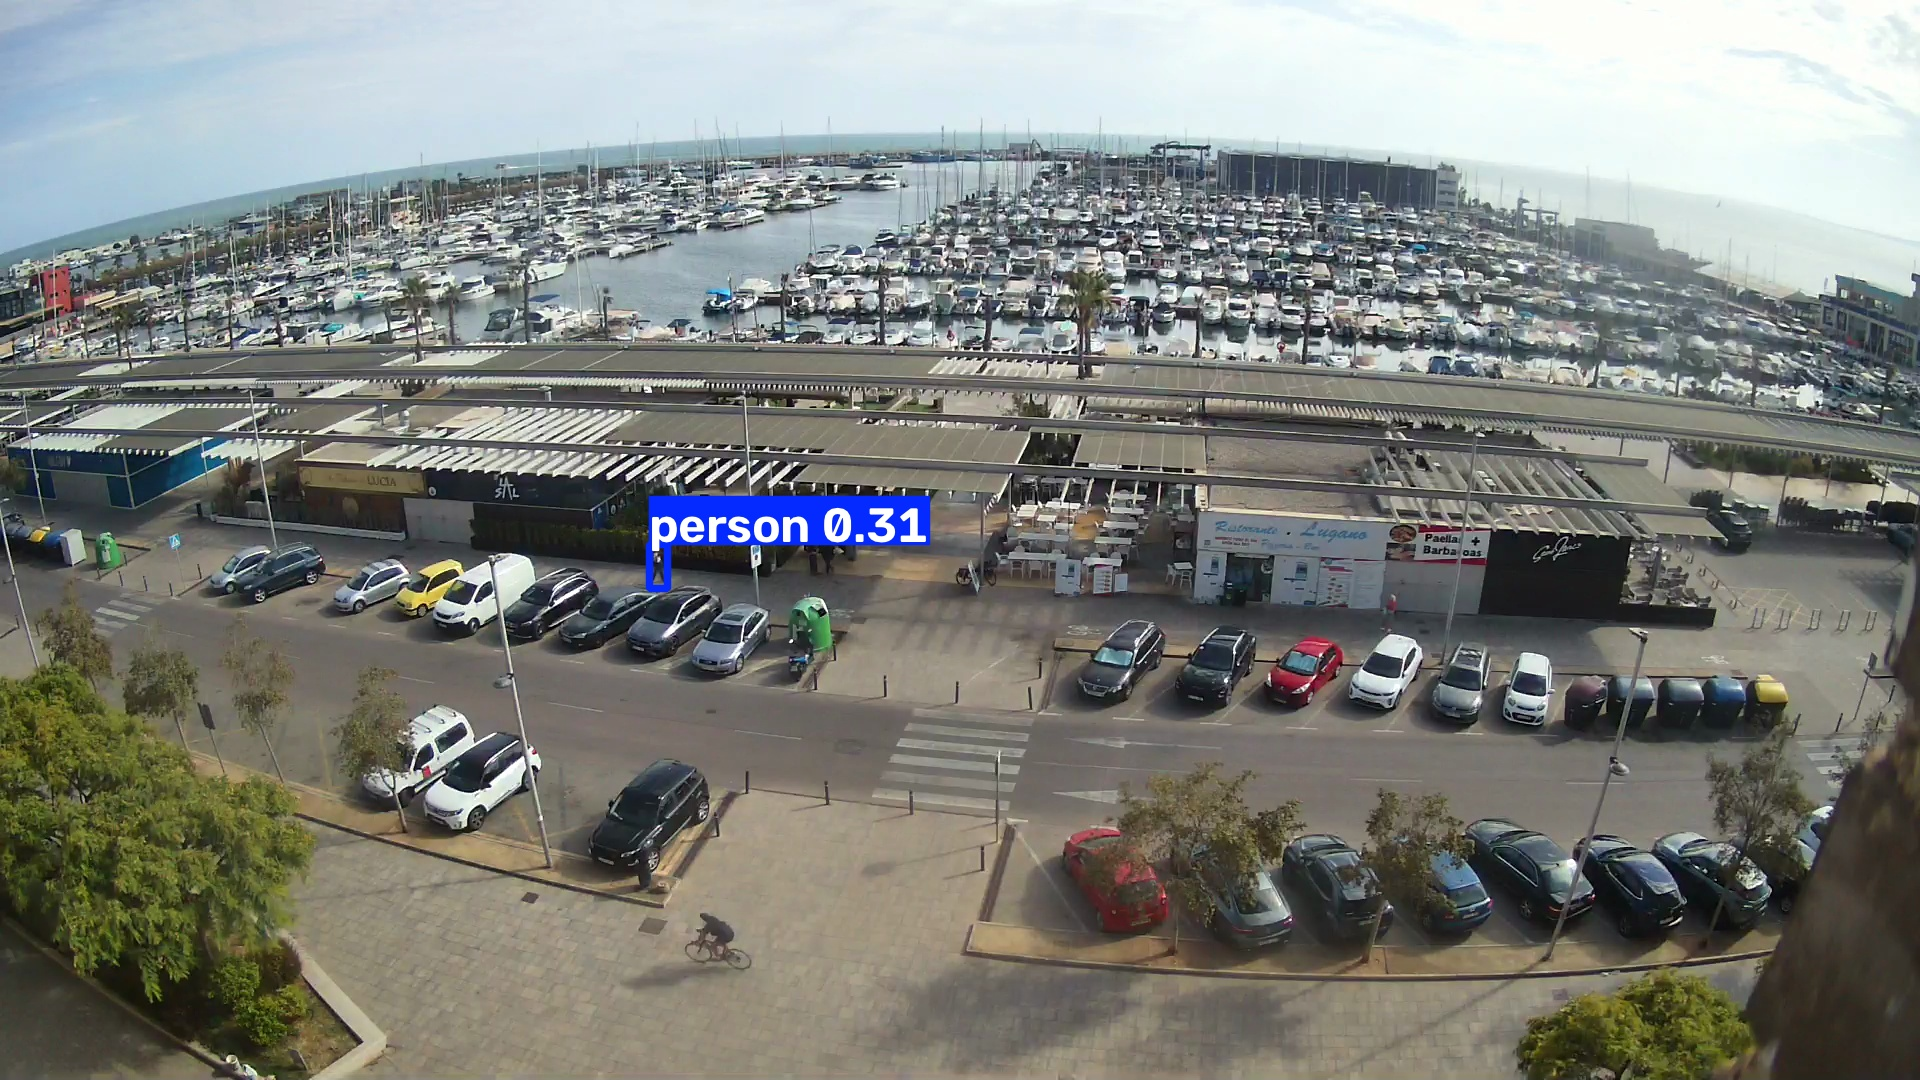
\includegraphics[width=0.9\textwidth]{images/part1_detection_example.jpg}
        \caption{Santa Pola webcam frame with a YOLOv8 person detection (confidence 0.31).}
        \label{fig:part1-detection}
    \end{figure}

    \begin{figure}[H]
        \centering
        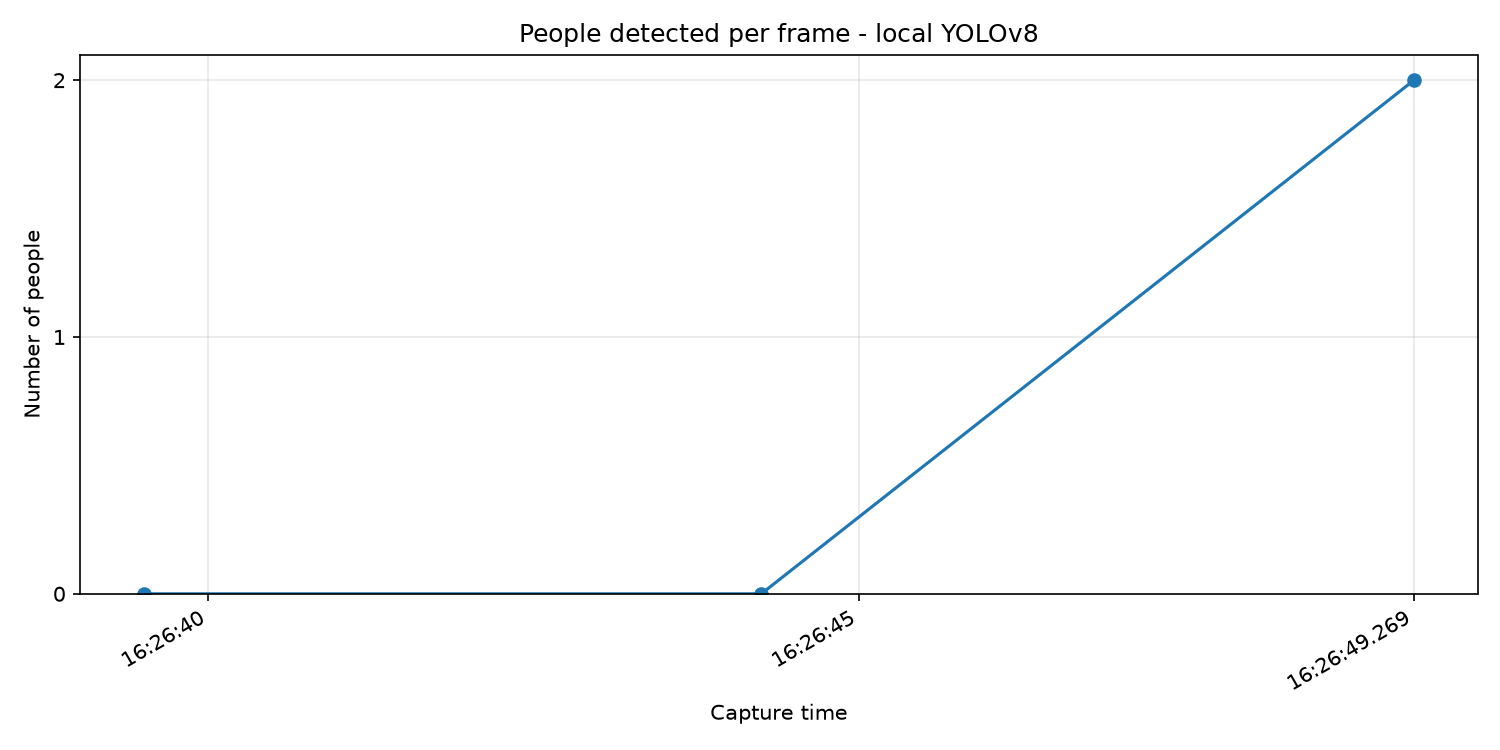
\includegraphics[width=0.9\textwidth]{images/part1_people_over_time.png}
        \caption{People detected in three consecutive webcam frames by local YOLOv8.}
        \label{fig:part1-plot}
    \end{figure}

    \subsection{Part 1 Conclusions}

    The local pipeline works end to end, including live capture, YOLOv8 person detection, CSV logging and graph generation. Increasing the inference size from 640 to 960 pixels improved detection of a distant person in the sample image, while keeping inference faster than at 1280 pixels in the limited comparison. This is a preliminary configuration choice, not a claim of measured accuracy. The three-frame Santa Pola run confirms the graph reflects the CSV data, but is too small to establish accuracy or sustained performance. We therefore kept Santa Pola for the initial VM implementation rather than changing the camera on this evidence alone; the more substantial VM false negatives and subsequent camera trial are described in Part 2.

\section{Part 2: Offloading to a Cloud Virtual Machine}
    \subsection{VM Creation and Setup (Task 2.1)}

    Part 2 uses the existing Azure virtual machine in Spain Central: Ubuntu 24.04, Standard B2ts v2, two virtual CPUs and 1 GiB of provisioned RAM (about 886 MiB available to the guest operating system). Figure~\ref{fig:part2-vm-overview} documents the VM's state, location and operating system in the Azure portal; Figure~\ref{fig:part2-vm-size} shows the selected size and its resources. Apache was already serving the public HTTP port. The deployment installs the Python service dependencies and a pinned headless OpenCV DNN build, then runs one Gunicorn worker with two threads as the \texttt{aiia-vm} system user. Apache forwards public requests to the Flask app listening only on \texttt{127.0.0.1:8765}; systemd starts and monitors the service. The pre-existing Apache welcome page is kept as a backup. No Azure network-security rules were changed.

    \begin{figure}[H]
        \centering
        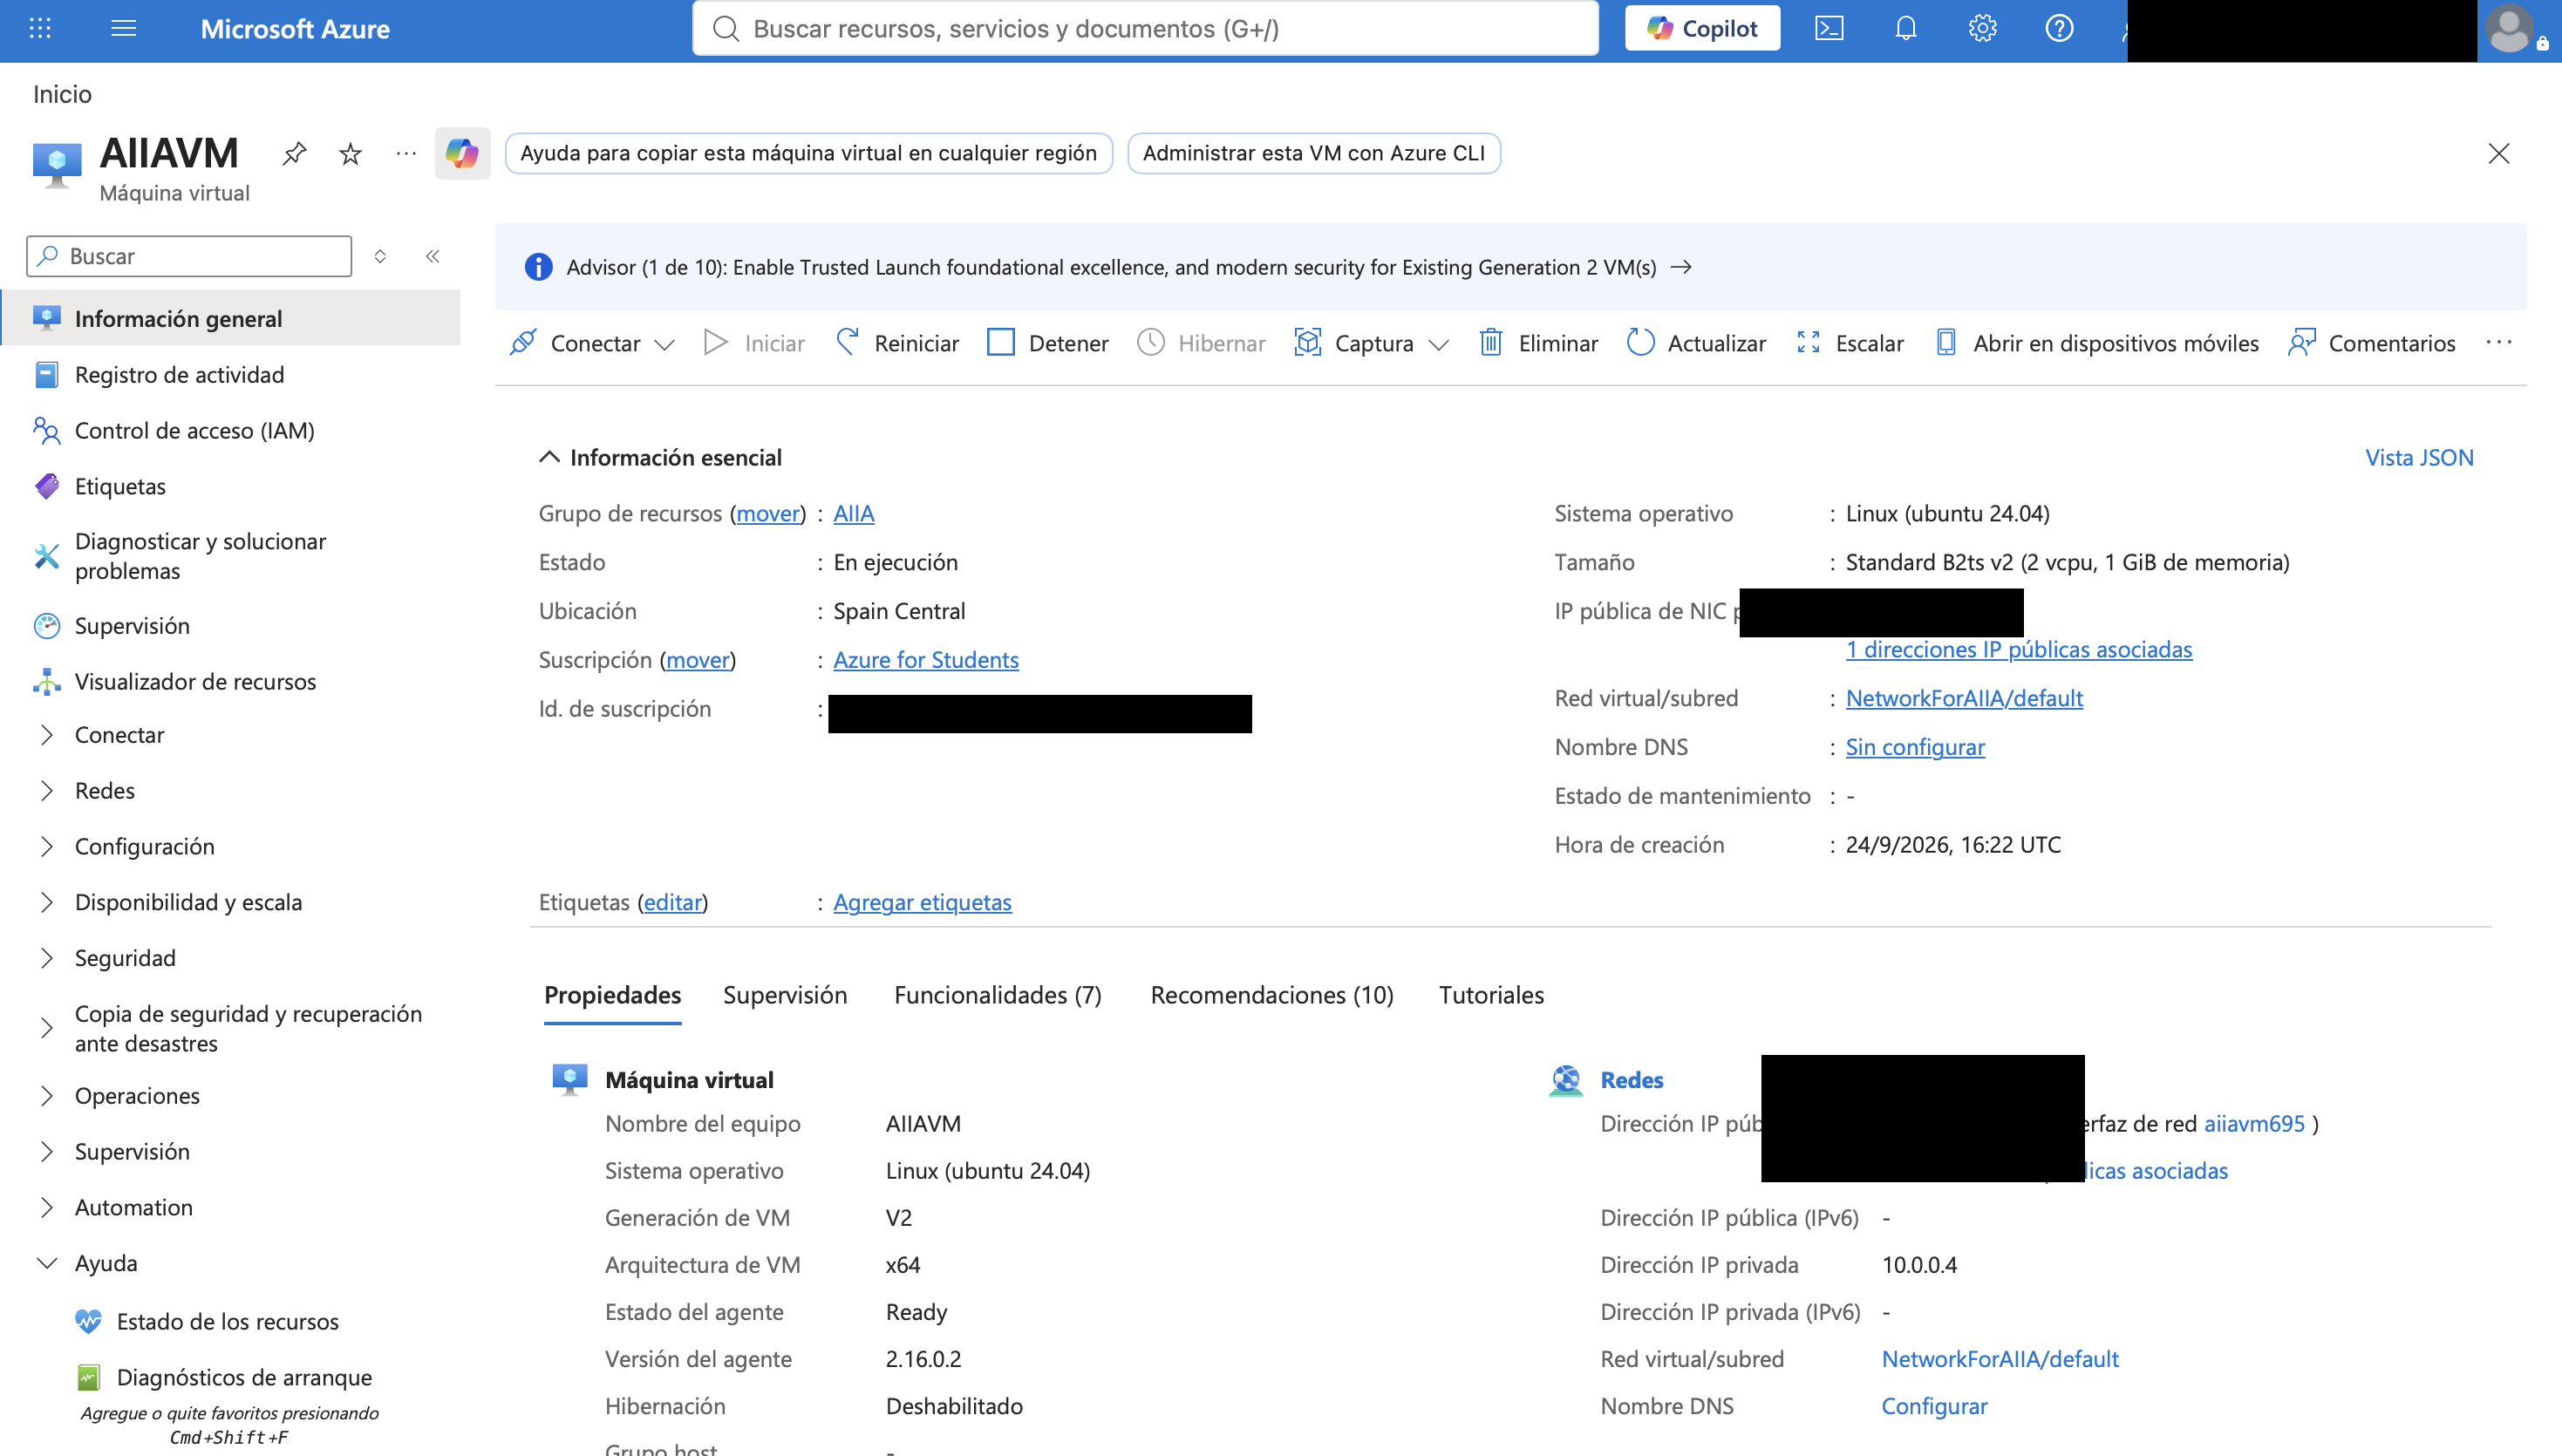
\includegraphics[width=0.98\textwidth]{images/part2_azure_vm_overview.png}
        \caption{Azure portal overview of the running AIIAVM, showing its region, Ubuntu version and VM size. The account email, subscription identifier and public IP address have been redacted.}
        \label{fig:part2-vm-overview}
    \end{figure}

    \begin{figure}[H]
        \centering
        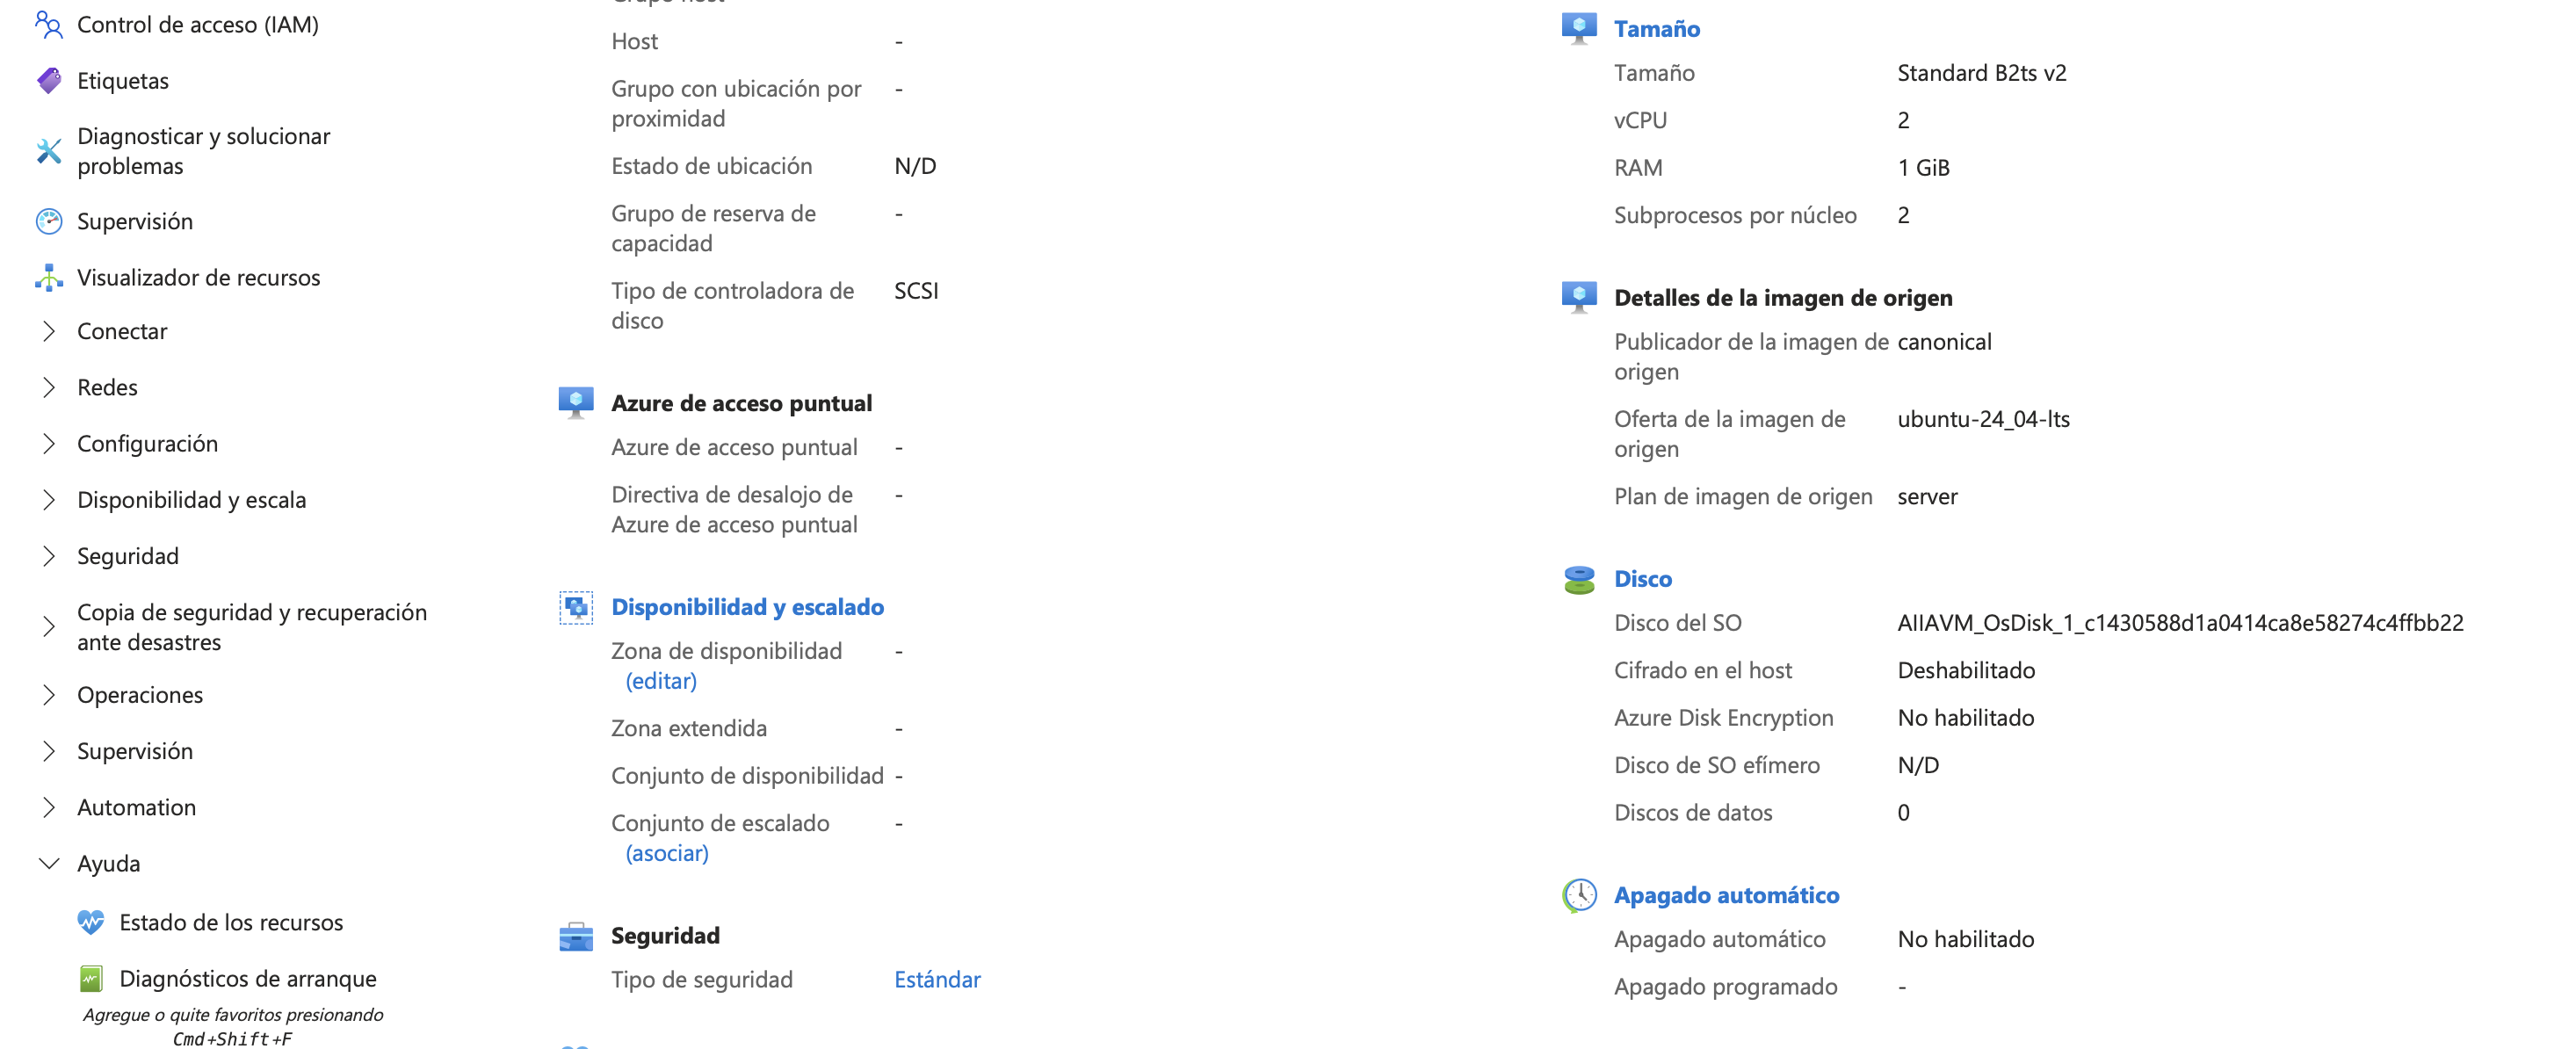
\includegraphics[width=0.98\textwidth]{images/part2_azure_vm_size.png}
        \caption{Azure portal properties confirming the Standard B2ts v2 size, two vCPUs and 1 GiB of RAM.}
        \label{fig:part2-vm-size}
    \end{figure}

    The YOLOv8 Nano weights are exported on the local computer to a static 960-pixel ONNX model, following the Ultralytics export workflow\footnote{\url{https://docs.ultralytics.com/modes/export/}}. This avoids installing PyTorch and Ultralytics on a VM with less than 1 GiB of RAM. The VM uses Python 3.12, NumPy 1.26.4 and OpenCV DNN 4.10.0.84\footnote{\url{https://docs.opencv.org/4.x/d6/d0f/group__dnn.html}}. A random bearer token protects frame uploads; its local configuration file is owner-readable only, and its server copy is root-owned with restricted group access.

    \paragraph{Problems encountered and design decisions.}
    Ubuntu's packaged OpenCV 4.6 could not parse an \texttt{Add} node in the exported ONNX graph. Pinning \texttt{opencv-python-headless} to 4.10.0.84 resolved the incompatibility. A deployment retry also exposed that recursive permission changes could remove executable bits from the virtual environment; the script now excludes it. After redeployment, systemd and Apache remained active throughout the ten-frame test.

    \subsection{Sending Frames to the VM (Task 2.2)}

    The local client reuses the shared capture module and sends one 1920$\times$1080 webcam frame every five seconds to \texttt{POST /api/frames}. Each request contains the camera identifier, the timezone-aware capture timestamp and a JPEG encoded at quality 85. The API accepts the image as a multipart upload and requires the bearer token. The first VM deployment used Santa Pola throughout, allowing the same camera to be tested locally and remotely.

    The endpoint validates the token, camera identifier, timestamp, JPEG format, image dimensions and request size before inference. The capture timestamp is included so that response time can be measured from the local capture through completion on the VM. This comparison assumes that the local computer and VM clocks are synchronized.

    \paragraph{Why we tested a second camera.}
    In the initial ten-frame Santa Pola VM performance run, YOLO returned zero people in five frames. Reviewing the corresponding webcam images showed that pedestrians were visible even in those zero-count frames. This was a concrete sign that the very wide, panoramic framing made distant people difficult to detect, rather than an issue with the upload or VM pipeline. We therefore kept the original Santa Pola results as the baseline and chose to test a less panoramic, more centred view: the SkylineWebcams plaza in Grazalema (Cádiz). We did not replace the input immediately; instead, we captured ten frames per camera using the same model and VM, then manually labelled both sets so their predicted counts could be compared with the visible people. The comparison and its limitations are reported in Task 2.5.

    \subsection{Processing on the VM (Task 2.3)}

    OpenCV DNN runs the exported YOLOv8n ONNX model on CPU. The input is letterboxed to 960$\times$960; detections are filtered to the COCO person class with confidence at least 0.25 and duplicate boxes are removed with non-maximum suppression at 0.45. The annotated frame is stored as \texttt{latest.jpg}. Each successful frame appends one row in the shared results format to \texttt{/var/lib/aiia-part2/results.csv}; CPU, process RSS, system RAM and uploaded JPEG bytes are recorded in \texttt{metrics.csv}.

    Across the 44 processed frames, YOLO returned 0 people eleven times, 1 person fifteen times, 2 people sixteen times and 3 people twice. The vehicle field is left empty because this implementation only detects people. Figure~\ref{fig:part2-histogram} previews the predicted-count distributions for the two-camera test; Task 2.5 explains why Grazalema was selected as the candidate and compares these predictions with manual counts. The VM result rows are preserved in \texttt{data/part2\_vm\_results.csv}.

    \begin{figure}[H]
        \centering
        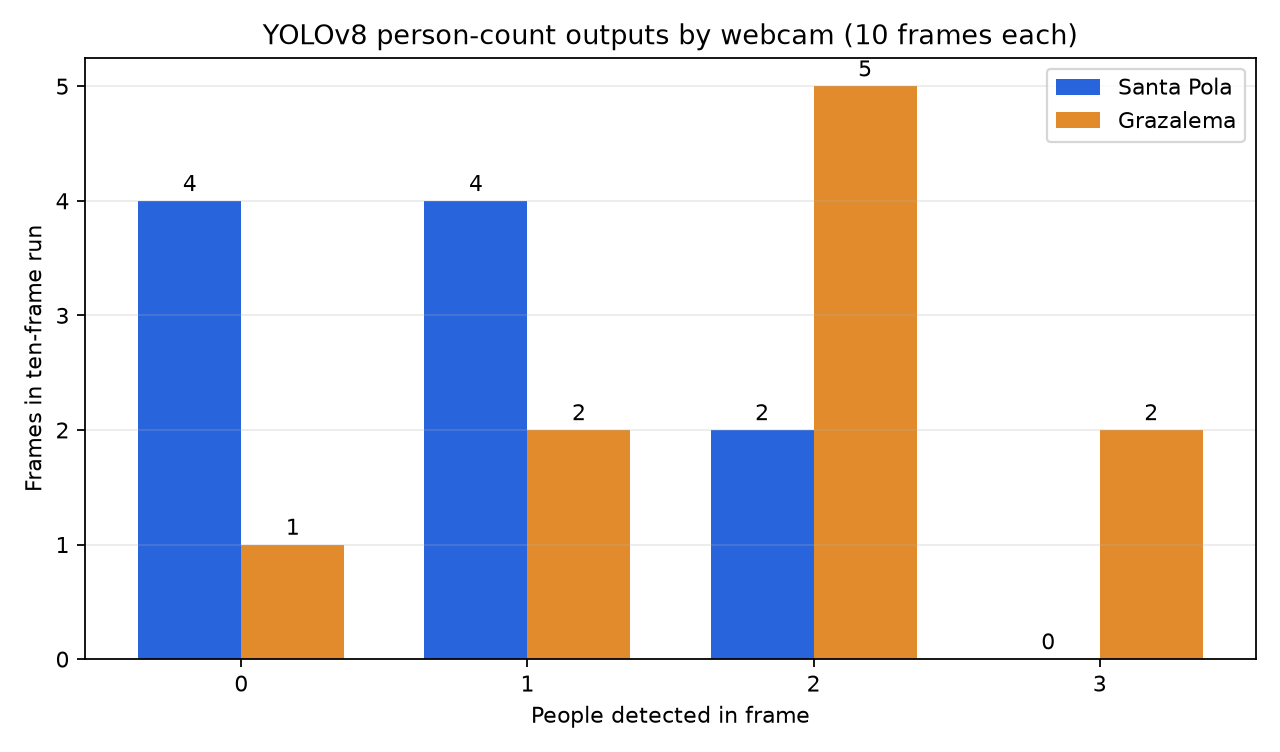
\includegraphics[width=0.76\textwidth]{images/part2_camera_comparison.png}
        \caption{YOLOv8 count outputs from ten-frame runs on Santa Pola and Grazalema. These are predicted-count distributions, not accuracy measurements.}
        \label{fig:part2-histogram}
    \end{figure}

    \subsection{Results Web Page (Task 2.4)}

    Apache publishes the dashboard on the VM's public IP address, \url{http://70.156.191.216/}. The page refreshes automatically and shows the people-count histogram, recent frame-level results, the latest image with person boxes when present, inference and response times, CPU, process and system memory, JPEG upload size and bandwidth, and an estimated compute cost. On 12 October 2026, both the public health endpoint and dashboard returned HTTP 200 after the new ten-frame upload run.

    Figures~\ref{fig:part2-dashboard-overview} and~\ref{fig:part2-dashboard-results} are browser captures of the live dashboard on 12 October 2026. At capture time, the VM had processed 45 frames; the cards showed a latest response of 1092.3 ms, process CPU of 94.4\%, process memory of 249.7 MB and a mean JPEG payload of 422.7 KiB per frame. The latest test frame had zero detections, while the accumulated histogram and recent-results table include earlier frames from both cameras. These are operational dashboard readings, not averages from the controlled ten-frame performance run in Table~\ref{tab:part2-performance}; the cost shown is the estimate accumulated since VM boot.

    \begin{figure}[H]
        \centering
        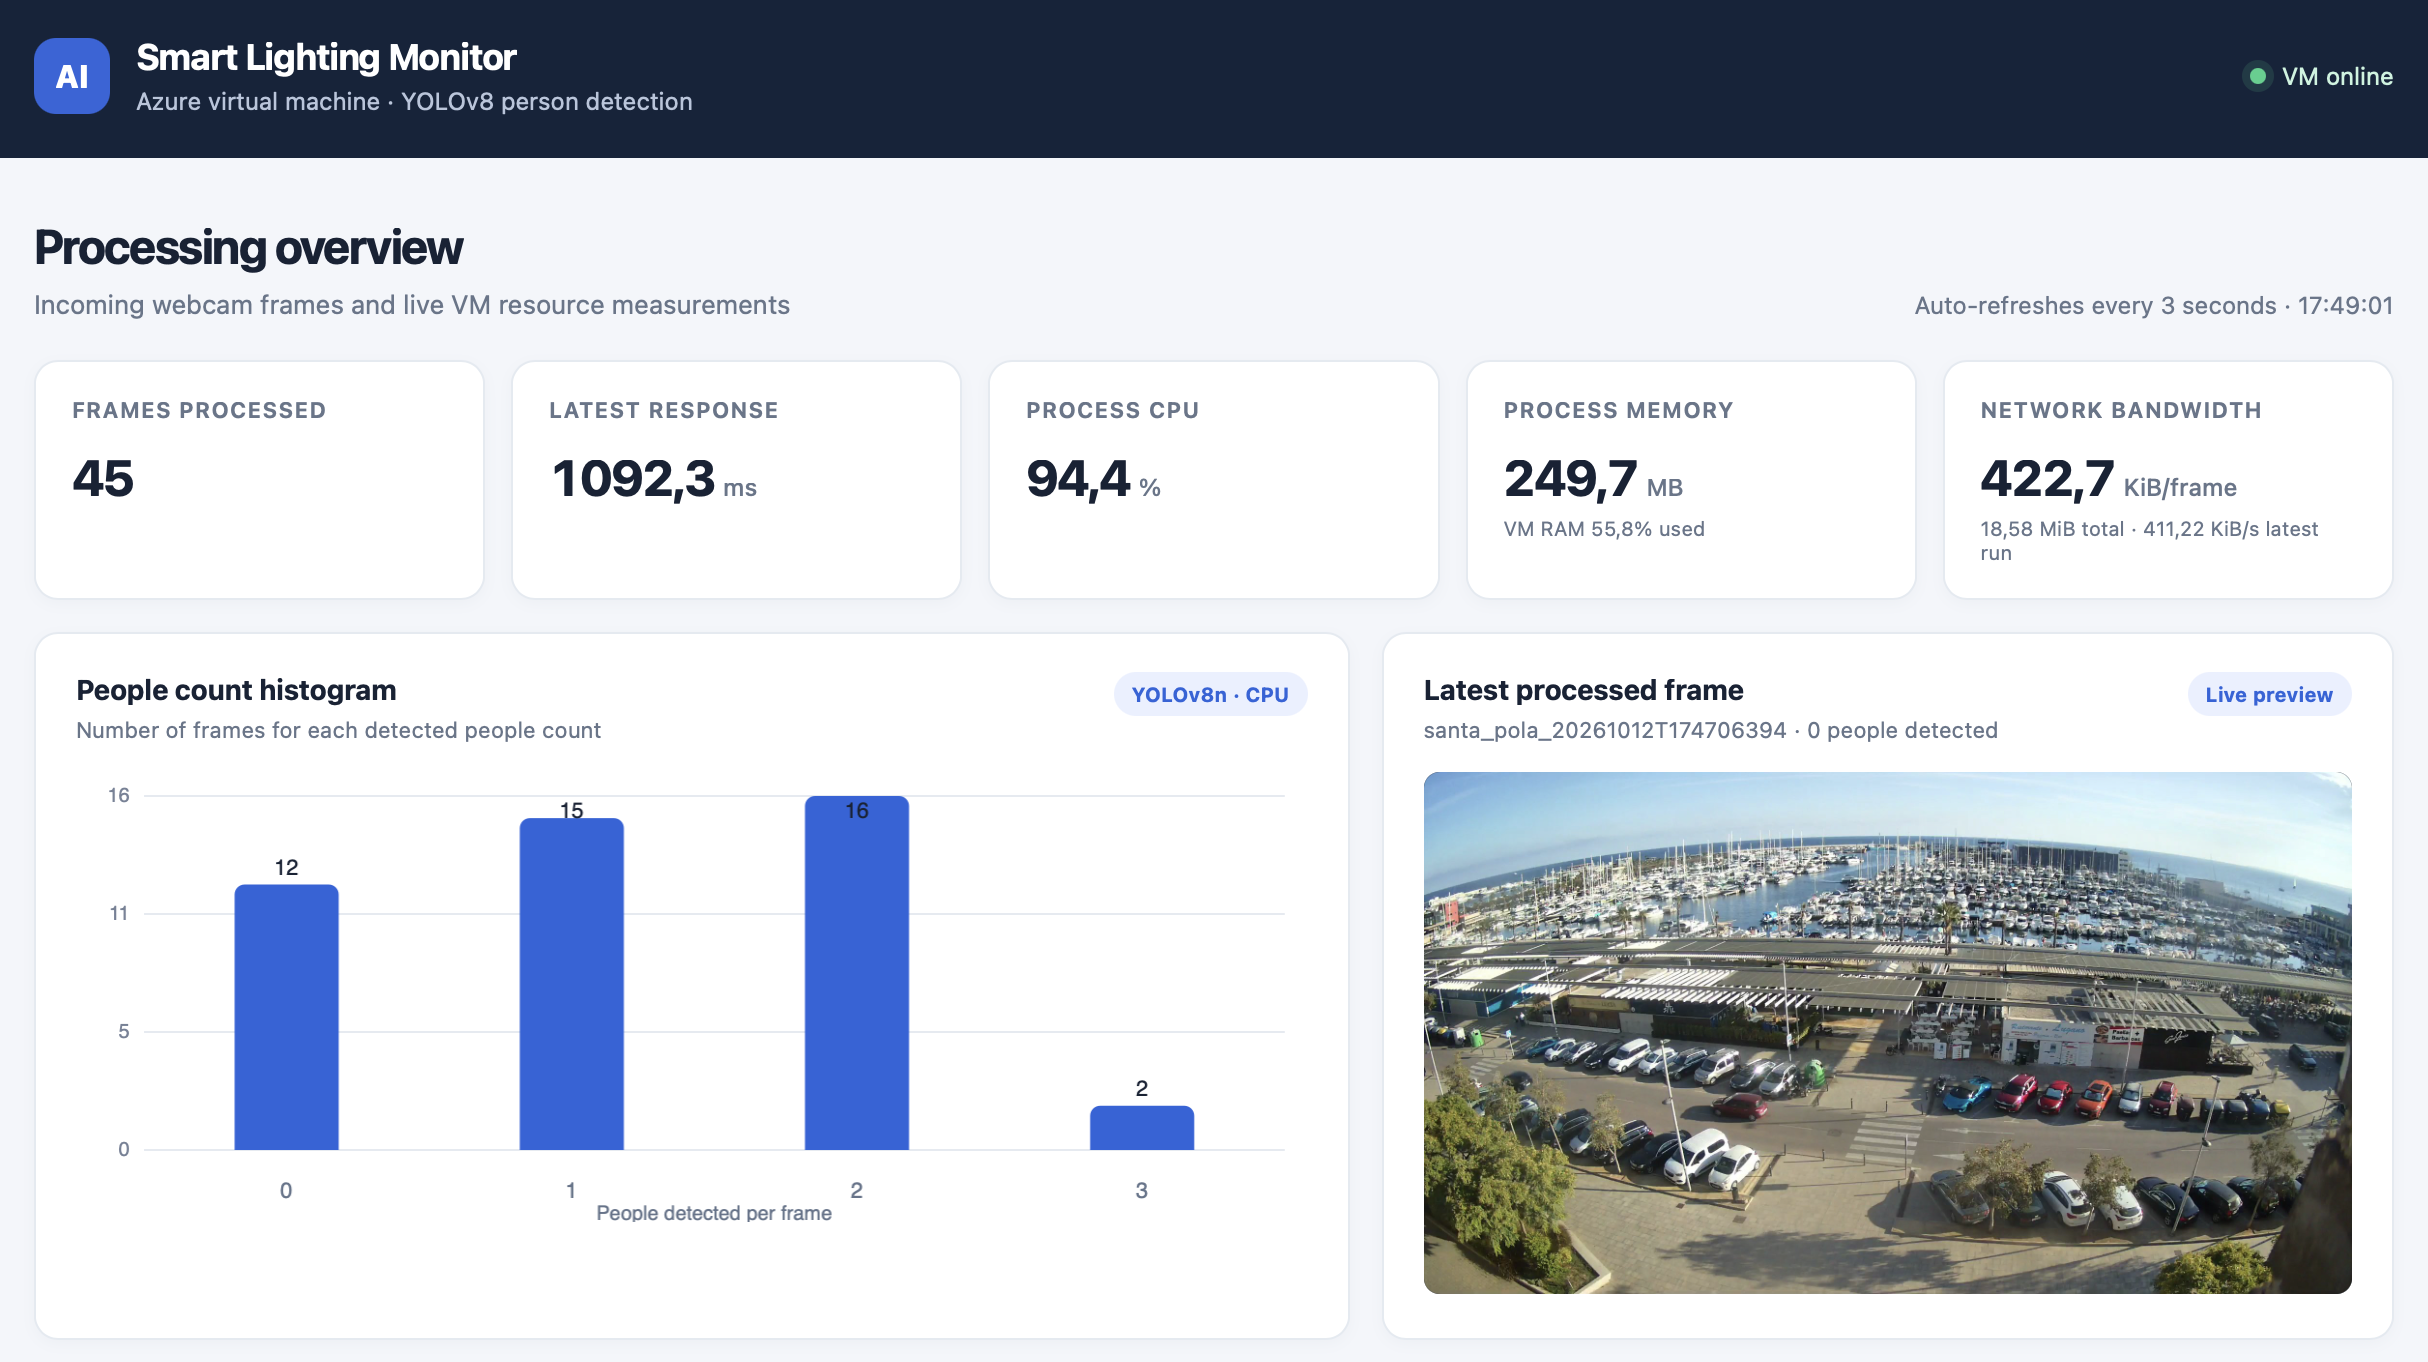
\includegraphics[width=0.98\textwidth]{images/part2_dashboard_overview.png}
        \caption{Dashboard overview after 45 frames, showing current VM measurements, the accumulated count histogram and the most recently processed frame.}
        \label{fig:part2-dashboard-overview}
    \end{figure}

    \begin{figure}[H]
        \centering
        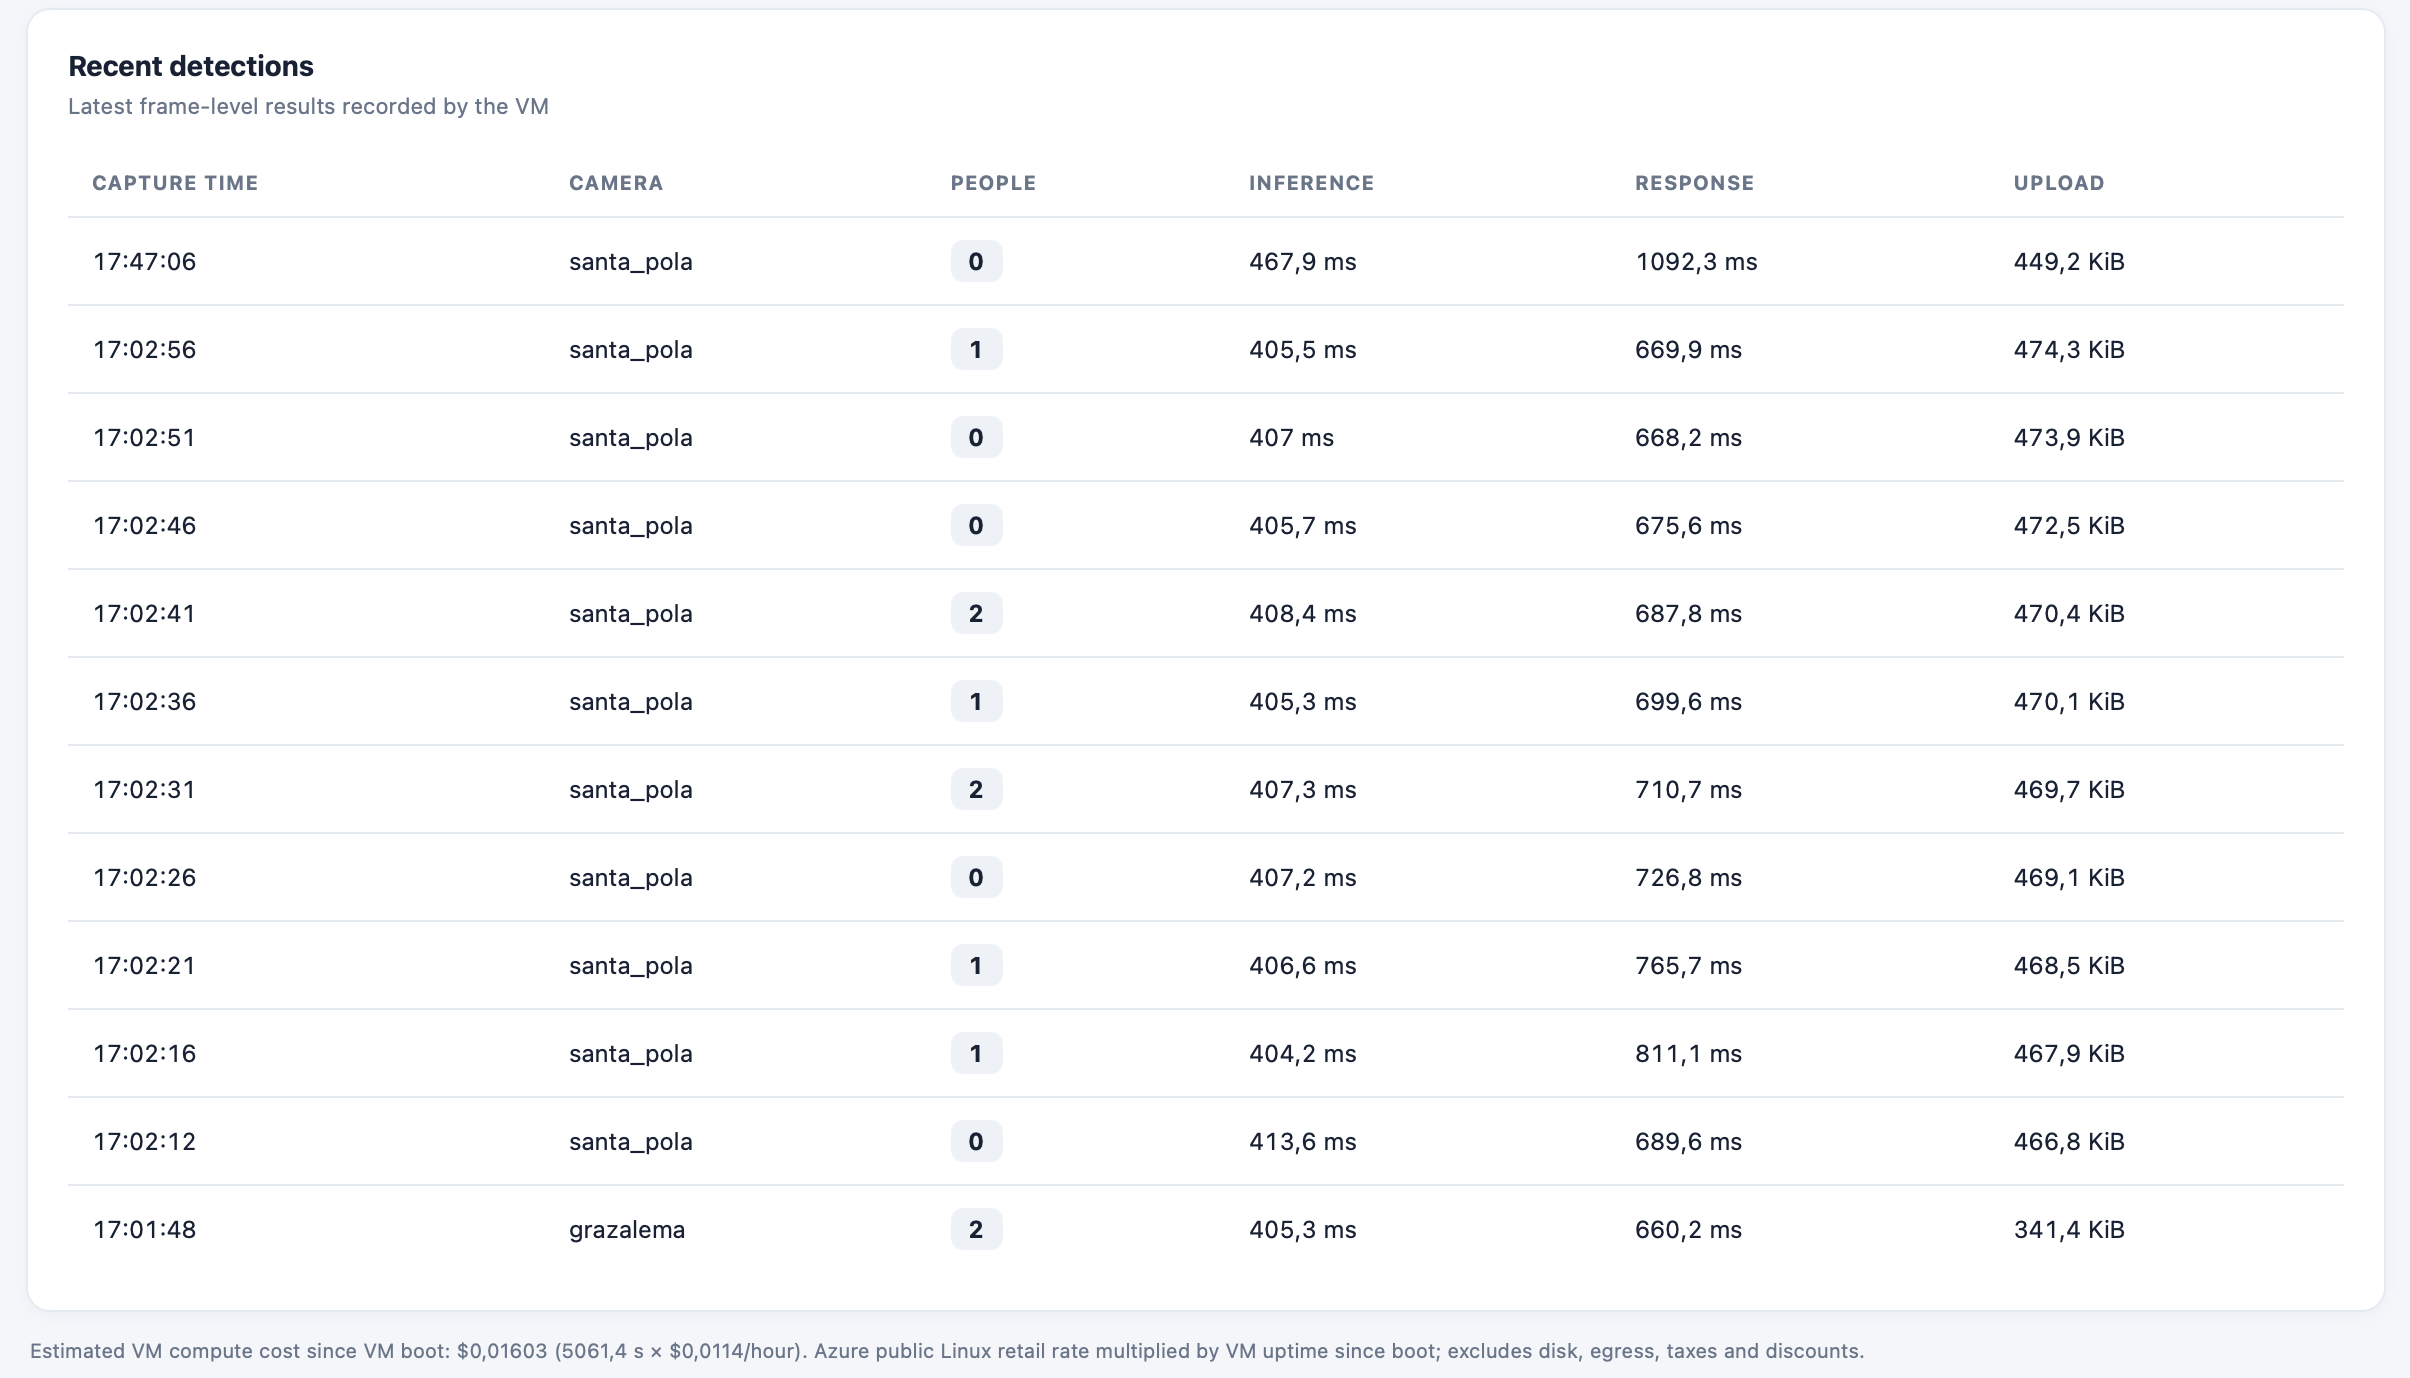
\includegraphics[width=0.98\textwidth]{images/part2_dashboard_detections.png}
        \caption{Dashboard recent-detections table and estimated compute cost, including records from the Santa Pola and Grazalema test runs.}
        \label{fig:part2-dashboard-results}
    \end{figure}

    Figure~\ref{fig:part2-preview} provides an example frame with a positive person detection; it is a previously processed Santa Pola frame, not the zero-detection frame displayed as the latest result in Figure~\ref{fig:part2-dashboard-overview}.

    \begin{figure}[H]
        \centering
        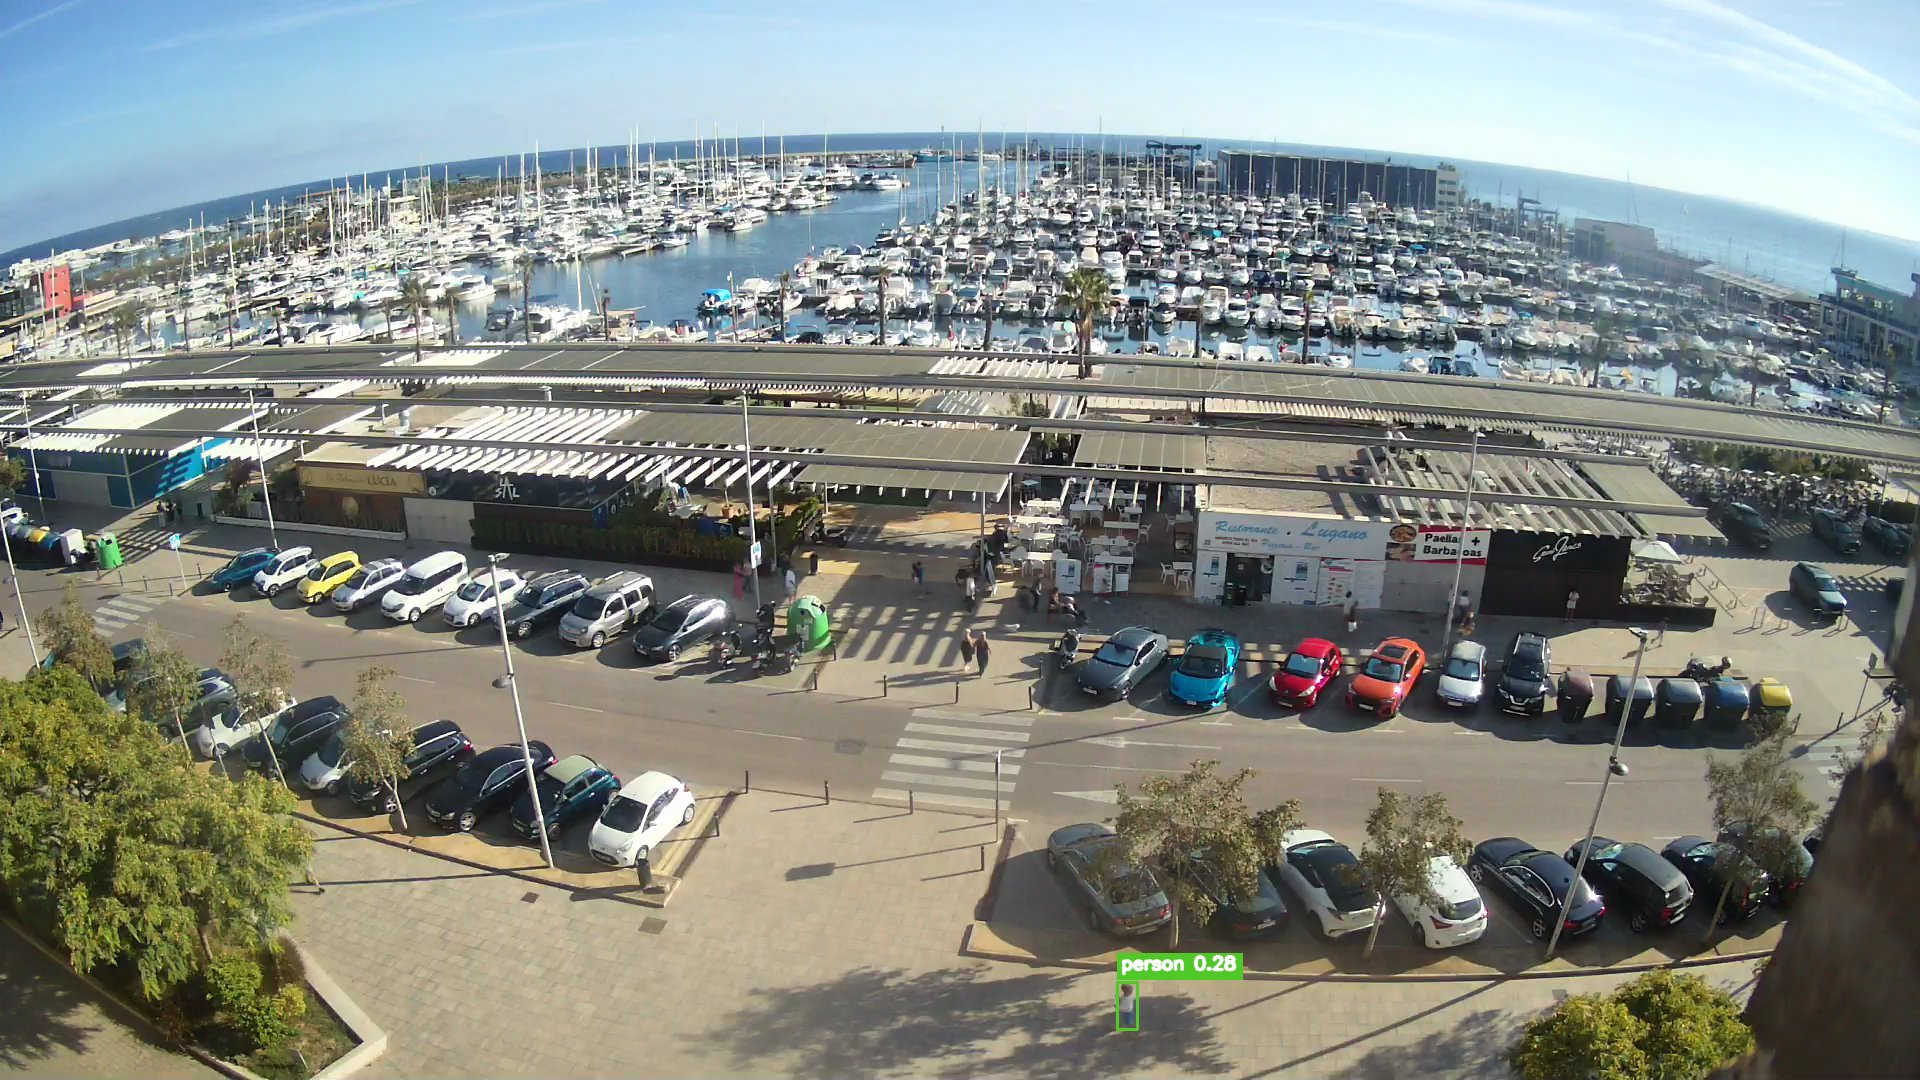
\includegraphics[width=0.9\textwidth]{images/part2_latest.jpg}
        \caption{Example previously processed Santa Pola frame with a YOLOv8 person detection overlaid.}
        \label{fig:part2-preview}
    \end{figure}

    The upload token is transmitted over HTTP in this course demonstration. It protects the endpoint from unauthenticated requests but does not encrypt the token or image in transit. A production deployment would require HTTPS and appropriate network restrictions.

    \subsection{Performance Analysis (Task 2.5)}

    The measured VM run on 12 October 2026 used the Santa Pola webcam at 1920$\times$1080, JPEG quality 85, one frame every five seconds, and CPU inference on the two-vCPU VM. The table reports these ten frames; the camera comparison below covers a separate ten-frame batch from each camera. Inference time measures the model forward pass; response time is the elapsed time from the local capture timestamp to completion on the VM. The system-RAM percentage and process RSS were sampled after each frame.

    \begin{table}[H]
        \centering
        \small
        \begin{tabular}{p{4.2cm}p{3.0cm}p{6.2cm}}
            \toprule
            \textbf{Metric} & \textbf{Observed result} & \textbf{Measurement and interpretation} \\
            \midrule
            Detection output & 10 frames: 5 with 0 and 5 with 1 person; all 44 frames: 11 with 0, 15 with 1, 16 with 2 and 2 with 3 & Predicted counts from the model. The separate labelled comparison is in Table~\ref{tab:camera-accuracy}. \\
            Inference time & 413.0 ms mean & Mean of the ten model forward-pass measurements. \\
            Response time & 792.8 ms mean; 732.0 ms median; 990.3 ms maximum & Capture-to-completion time, including network transfer and server processing; clocks must be synchronized. All ten responses finished within the five-second capture interval. \\
            CPU & 95.6\% mean; 96.9\% maximum & Process CPU use normalized over the VM's two logical CPUs during request processing. This is high utilization for the tested workload. \\
            Process memory & 271.9 MB mean; 273.4 MB maximum & Resident set size sampled for the inference service during the ten-frame run. \\
            VM memory & 57.4\% maximum of about 886 MiB & System-wide RAM percentage from \texttt{psutil}; the VM had no swap configured. \\
            Upload payload & 4.92 MiB total; 503.5 KiB per frame on average & Sum and mean of the ten encoded JPEG request bodies. \\
            Payload rate & 110.9 KiB/s & JPEG payload divided by 45.38 seconds from the first capture through completion of the last result. Network-interface counters also include unrelated VM traffic. \\
            Estimated compute cost & \$0.0001437 for 45.38 s & Calculated at the public Linux retail rate of \$0.0114/hour for this SKU and region. This short-window estimate excludes disk, egress, taxes and discounts and is not an Azure invoice amount. \\
            \bottomrule
        \end{tabular}
        \caption{VM performance for the ten-frame run on 12 October 2026 at five-second capture intervals.}
        \label{tab:part2-performance}
    \end{table}

    The service kept up with one camera at the configured interval: all ten responses completed in less than one second, below the five-second interval. CPU remained close to full use during frame processing, so the VM may have limited headroom for additional cameras; multi-camera capacity is assessed separately in Part 4. The ONNX service used about 272 MB of process memory on average, which is materially smaller than loading the full PyTorch stack would require on this VM.

    To evaluate detection effectiveness, all 20 frames in the two comparison batches were labelled manually by counting the visible people in each frame. The labels, model outputs and frame paths are preserved in \texttt{data/part2\_vm\_ground\_truth.csv}; \texttt{local\_vm/evaluate\_vm\_counts.py} computes metrics overall and separately per camera. Exact-count accuracy means that the predicted number exactly matches the manual count. MAE and RMSE measure the absolute count error in people per frame; signed bias is prediction minus ground truth, so a negative value means undercounting.

    \begin{table}[H]
        \centering
        \small
        \begin{tabular}{lrrrrrr}
            \toprule
            \textbf{Camera} & \textbf{Frames} & \textbf{Exact (\%)} & \textbf{MAE} & \textbf{RMSE} & \textbf{Bias} & \textbf{Under-count} \\
            \midrule
            Santa Pola & 10 & 0\% & 5.9 & 6.19 & -5.9 & 10/10 \\
            Grazalema & 10 & 20\% & 1.7 & 2.02 & -1.7 & 8/10 \\
            Combined & 20 & 10\% & 3.8 & 4.60 & -3.8 & 18/20 \\
            \bottomrule
        \end{tabular}
        \caption{Frame-level person-count comparison against manually labelled ground truth. MAE, RMSE and bias are people per frame; under-count is the number of frames with a negative prediction error.}
        \label{tab:camera-accuracy}
    \end{table}

    In this labelled sample, YOLO undercounted in 18 of 20 frames and never overcounted. Grazalema had lower count error than Santa Pola (MAE 1.7 versus 5.9 people/frame) and higher exact-count agreement (20\% versus 0\%). This provides evidence that Grazalema is the better of these two camera/model combinations for the observed samples, consistent with the denser framing; it does not establish general accuracy because the evaluation covers only ten frames per camera at one time of day. Exact-count accuracy, MAE and RMSE measure frame counts and should not be interpreted as box-level precision or recall. The substantial undercounting on both cameras also means that changing cameras alone does not make this YOLO configuration sufficiently reliable for deployment without further tuning and evaluation.

    The table's cost is a short-window estimate based on a public retail compute rate, not measured subscription billing. The \$0.0114/hour rate was looked up through the Azure Retail Prices API\footnote{\url{https://prices.azure.com/api/retail/prices}}. The deployed dashboard now estimates cumulative compute cost from VM uptime since the latest OS boot; the refreshed public API snapshot in \texttt{part2\_dashboard.json} confirms the updated cost basis and measured uptime. This is still an estimate, not an Azure invoice, and excludes disk, egress, taxes and subscription discounts. The dashboard also computes payload throughput for the latest uninterrupted run, excluding pauses longer than 60 seconds; the eleven-day gap between the two runs is no longer counted. The short-window cost and payload rate in Table~\ref{tab:part2-performance} are calculated directly from the ten-frame run.

    \subsection{Exploratory Camera Comparison}

    Following the false negatives in the initial Santa Pola VM run, the Grazalema plaza was chosen as a candidate because its view is less panoramic and more centred on the pedestrian area. To test the decision rather than assume it helped, ten frames from each camera were uploaded to the same VM on 12 October 2026. Capture interval (5 s), JPEG quality (85), YOLOv8n ONNX weights, 960-pixel input, confidence threshold (0.25), NMS threshold (0.45) and VM were kept constant. The Grazalema run was captured from 17:01:03 to 17:01:48; Santa Pola was captured immediately afterward, from 17:02:12 to 17:02:56. The 44 result rows, including both comparison batches and the initial VM tests, are in \texttt{data/part2\_vm\_results.csv}.

    \begin{table}[H]
        \centering
        \small
        \begin{tabular}{lrrrrrr}
            \toprule
            \textbf{Camera} & \textbf{Frames} & \textbf{0 people} & \textbf{1 person} & \textbf{2 people} & \textbf{3 people} & \textbf{Mean detections/frame} \\
            \midrule
            Santa Pola & 10 & 4 & 4 & 2 & 0 & 0.8 \\
            Grazalema & 10 & 1 & 2 & 5 & 2 & 1.8 \\
            \bottomrule
        \end{tabular}
        \caption{YOLOv8 predicted-count distributions for the two latest ten-frame camera runs.}
        \label{tab:camera-comparison}
    \end{table}

    On this sample, Grazalema produced 1.8 detections per frame on average versus 0.8 for Santa Pola, while mean inference time was similar (413 ms versus 407 ms). The average encoded JPEG was smaller for Grazalema (342 KiB versus 470 KiB). Since the scenes contain different numbers of actual people and the runs were sequential, predictions alone cannot demonstrate an improvement. The manual frame-count labels in Table~\ref{tab:camera-accuracy} do show lower count error for Grazalema in these samples, though both cameras still exhibit substantial undercounting. The example in Figure~\ref{fig:camera-scenes} shows the less panoramic and more centred Grazalema view that motivated the trial, but people can still be small, shaded or occluded. The measured result justifies selecting Grazalema as the preferred input for subsequent experiments, not treating the detector as accurate or claiming general superiority. Both camera URLs remain available through \texttt{--cam}.

    \begin{figure}[H]
        \centering
        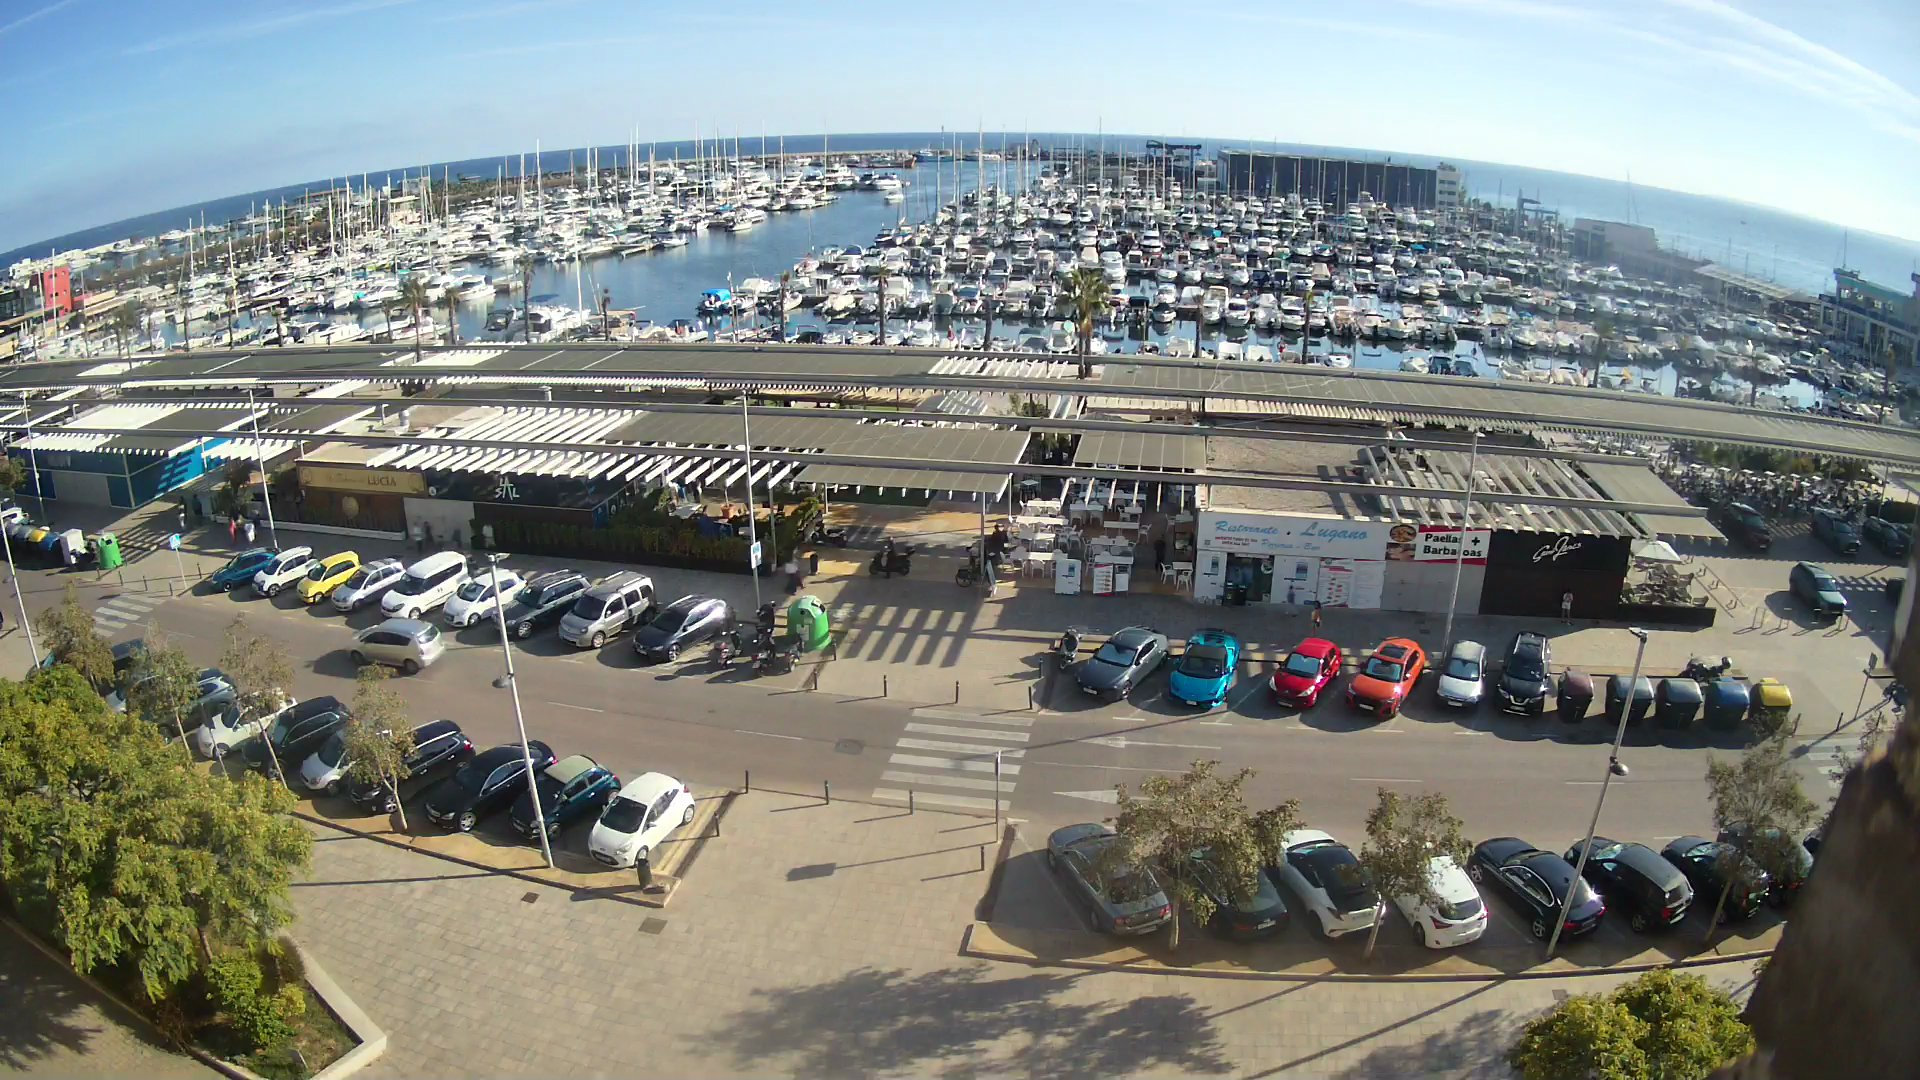
\includegraphics[width=0.49\textwidth]{part2_frames/santa_pola_20261012T170212091.jpg}
        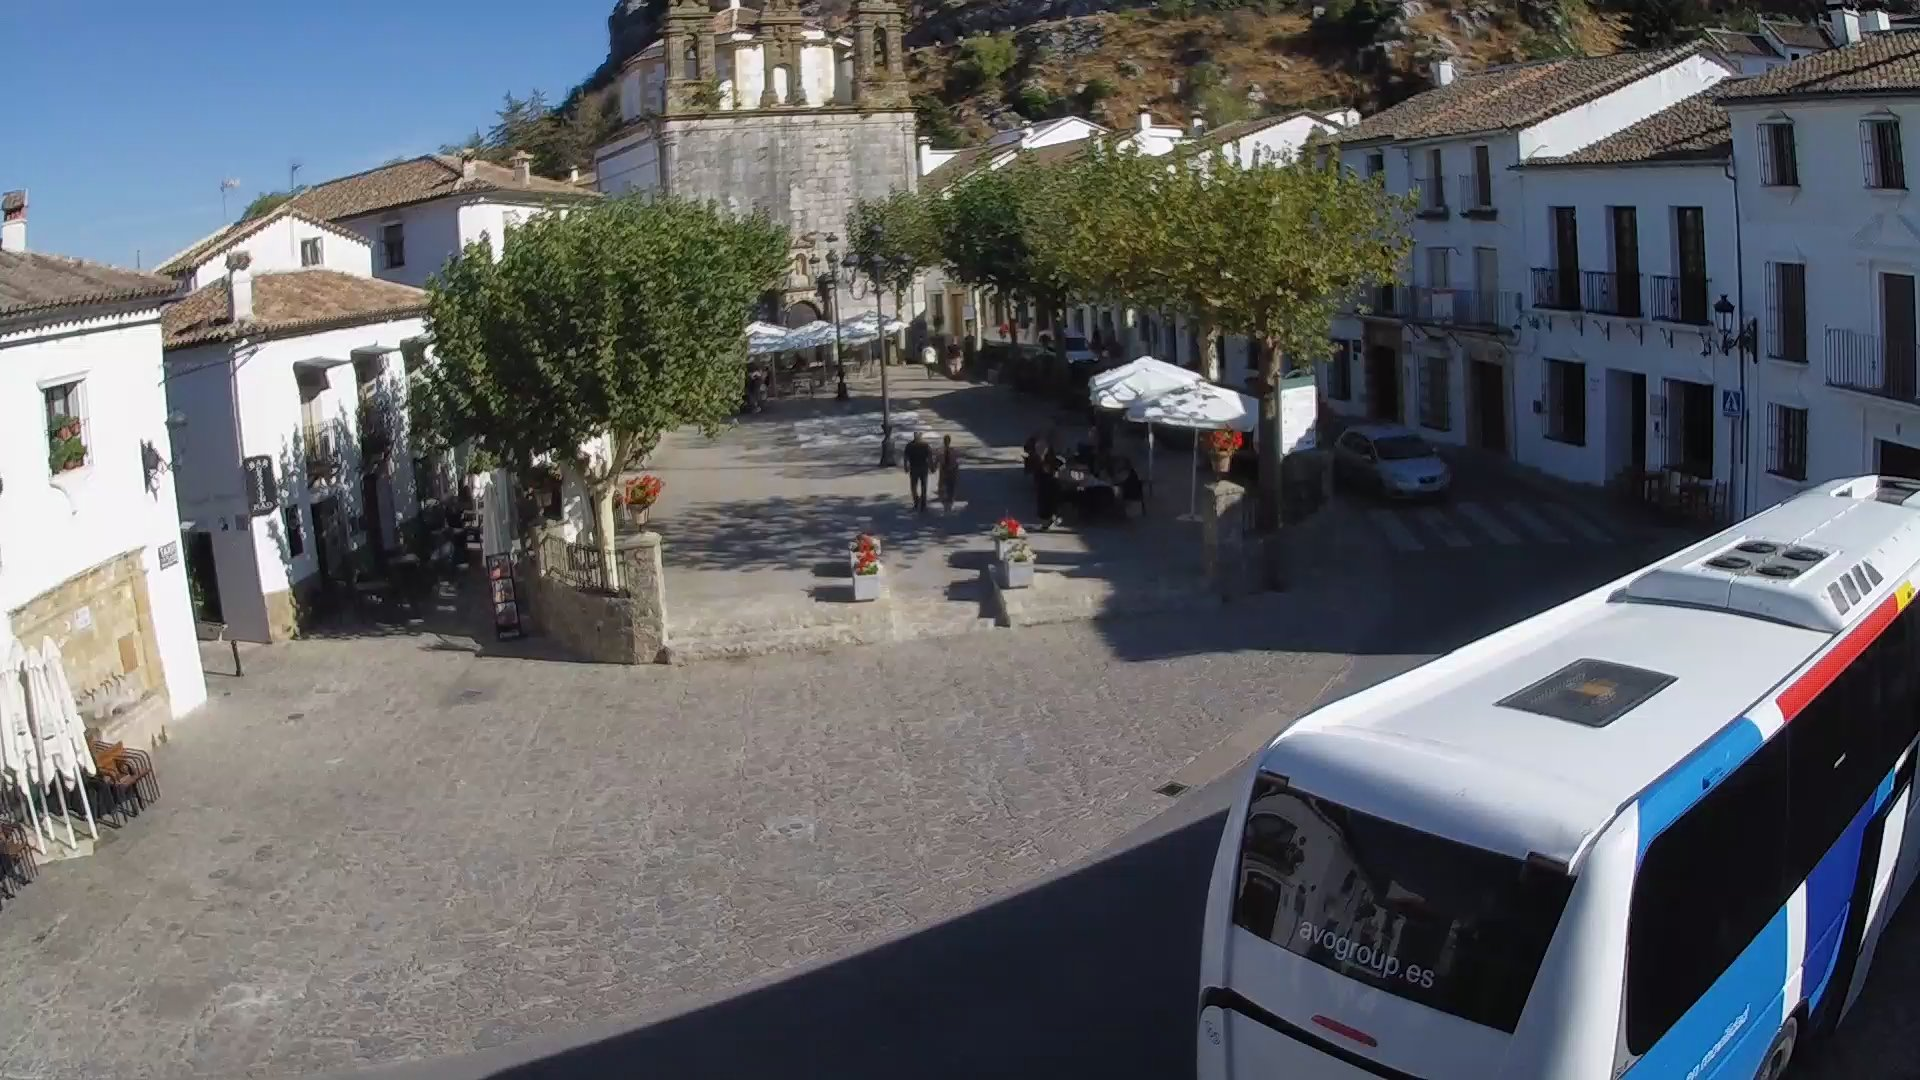
\includegraphics[width=0.49\textwidth]{part2_frames/grazalema_20261012T170103889.jpg}
        \caption{Example frames from the comparison: Santa Pola (left) and Grazalema (right), captured within about one minute.}
        \label{fig:camera-scenes}
    \end{figure}

    \subsection{Part 2 Conclusions}

    The local-to-VM pipeline is operational end to end: live webcam frames are authenticated and uploaded, processed with YOLOv8 on the VM, recorded in the shared CSV format and shown on a publicly accessible dashboard. Exporting ONNX and using a pinned OpenCV DNN runtime made deployment feasible on the VM's limited memory. In the latest ten-frame Santa Pola test, all responses completed within one second, while CPU utilization remained high and process memory averaged 272 MB. The labelled ten-frame comparison found lower count error on Grazalema (MAE 1.7 versus 5.9 people/frame), supporting it as the preferred camera for further testing. However, the model undercounted in 18/20 labelled frames across both views, so improved framing does not resolve the detector's reliability limitation; longer representative tests and model/configuration improvements are still needed. Multi-camera capacity remains a separate limitation.

\section{Part 3: Serverless Architecture}
    \subsection{Static Website on Azure Storage (Task 3.1)}
    \subsection{Uploading Frames to the Raw Container (Task 3.2)}
    \subsection{Azure AI Vision Service (Task 3.4)}
    \subsection{Blob-Triggered Function (Task 3.3 and 3.5)}
    \subsection{Performance Analysis (Task 3.6)}
    \subsection{Part 3 Conclusions}

    Pending: conclusions will be added after the serverless workflow has been deployed and its processing and performance have been measured.

\section{Part 4: Multi-Camera Management}
    \subsection{Additional Camera Selection (Task 4.1)}
    \subsection{VM Scalability (Task 4.2)}
    \subsection{Serverless Scalability (Task 4.3)}
    \subsection{Part 4 Conclusions}

    Pending: conclusions will be added after the multi-camera tests have been run and the architectures' scaling limits have been compared.

\section{Advanced Tasks}
    \subsection{Unique Person Counting (Tracking)}
    \subsection{Person and Vehicle Counting}
    \label{sec:vehicles}
    \subsection{Performance Optimizations}
    \subsection{Advanced Tasks Conclusions}

    Pending: conclusions will be added after the advanced features and their optimizations have been implemented and evaluated.

\section{Architecture Comparison}                  % local vs VM vs serverless table
\section{Conclusions}

Parts 1 and 2 demonstrate a working local and VM-based capture, inference and results pipeline. The VM deployment shows that ONNX with OpenCV DNN can run within the memory limits of the selected Azure size, but CPU use is high and the labelled count comparison reveals substantial undercounting, particularly for the panoramic Santa Pola view. Grazalema performed better in the small labelled sample, but neither camera/model combination is accurate enough to treat the count as reliable without further evaluation and tuning.

These findings are limited to the measured samples and do not establish performance under other times, lighting conditions or camera loads. The overall comparison and final conclusions remain incomplete because Parts 3 and 4 have not yet been documented with results; the corresponding report sections are explicitly marked as pending.

\section{References}

\begin{enumerate}
    \item SkylineWebcams, Santa Pola -- Paseo Marítimo. \href{https://www.skylinewebcams.com/es/webcam/espana/comunidad-valenciana/santa-pola/paseo-maritimo.html}{Camera page}
    \item SkylineWebcams, Grazalema. \href{https://www.skylinewebcams.com/es/webcam/espana/andalucia/cadiz/grazalema.html}{Camera page}
    \item Ultralytics, YOLOv8 model export documentation. \href{https://docs.ultralytics.com/modes/export/}{Export documentation}
    \item OpenCV, Deep Neural Network module documentation. \href{https://docs.opencv.org/4.x/d6/d0f/group__dnn.html}{DNN documentation}
    \item Microsoft Learn, Azure B-series burstable virtual machine sizes. \href{https://learn.microsoft.com/azure/virtual-machines/sizes/general-purpose/b-series}{B-series sizes}
    \item Microsoft Azure, Retail Prices API. \href{https://prices.azure.com/api/retail/prices}{API reference}
\end{enumerate}

Web resources accessed on 12 October 2026.
\appendix
\section{Deployment Details}                       % commands, configuration (optional)


\end{document}
